% Soubory musí být v kódování, které je nastaveno v příkazu \usepackage[...]{inputenc}

\documentclass[%        Základní nastavení
%  draft,    				  % Testovací překlad
  12pt,       				% Velikost základního písma je 12 bodů
  a4paper,    				% Formát papíru je A4
  oneside,      			% Jednostranný tisk
	%twoside,      			% Dvoustranný tisk (kapitoly a další důležité části tedy začínají na lichých stranách)
	unicode,						% Záložky a metainformace ve výsledném  PDF budou v kódování unicode
]{report}				    	% Dokument třídy 'zpráva', vhodná pro sazbu závěrečných prací s kapitolami

\usepackage[utf8]		  %	Kódování zdrojových souborů je UTF-8
	{inputenc}					% Balíček pro nastavení kódování zdrojových souborů

\usepackage[				% Nastavení geometrie stránky
	bindingoffset=10mm,		% Hřbet pro vazbu
	hmargin={25mm,25mm},	% Vnitřní a vnější okraj
	vmargin={25mm,34mm},	% Horní a dolní okraj
	footskip=17mm,			  % Velikost zápatí
	nohead,					      % Bez záhlaví
	marginparsep=2mm,		  % Vzdálenost marginálií
	marginparwidth=18mm,	% Šířka marginálií
]{geometry}
\usepackage{siunitx}
\usepackage{sectsty}
	%přetypuje nadpisy všech úrovní na bezpatkové, kromě \chapter, která je přenastavena zvlášť v thesis.sty
	\allsectionsfont{\sffamily}

\usepackage{graphicx} % Balíček 'graphicx' pro vkládání obrázků
											% Nutné pro vložení logotypů školy a fakulty

\usepackage[          % Balíček 'acronym' pro sazby zkratek a symbolů
	nohyperlinks				% Nebudou tvořeny hypertextové odkazy do seznamu zkratek
]{acronym}						
											% Nutné pro použití prostředí 'acronym' balíčku 'thesis'

\usepackage[
	breaklinks=true,		% Hypertextové odkazy mohou obsahovat zalomení řádku
	hypertexnames=false % Názvy hypertext. odkazů budou tvořeny nezávisle na názvech TeXu
]{hyperref}						% Balíček 'hyperref' pro sazbu hypertextových odkazů
											% Nutné pro použití příkazu 'pdfsettings' balíčku 'thesis'

\usepackage{pdfpages} % Balíček umožňující vkládat stránky z PDF souborů
                      % Nutné při vkládání titulních listů a zadání přímo
                      % ve formátu PDF z informačního systému

\usepackage{enumitem} % Balíček pro nastavení mezerování v odrážkách
  \setlist{topsep=0pt,partopsep=0pt,noitemsep} % konkrétní nastavení

\usepackage{cmap} 		% Balíček cmap zajišťuje, že PDF vytvořené `pdflatexem' je
											% plně "prohledávatelné" a "kopírovatelné"

%\usepackage{upgreek}	% Balíček pro sazbu stojatých řeckých písmem
											%% např. stojaté pí: \uppi
											%% např. stojaté mí: \upmu (použitelné třeba v mikrometrech)
											%% pozor, grafická nekompatibilita s fonty typu Computer Modern!
                      
%\usepackage{amsmath} %balíček pro sabu náročnější matematiky                 

\usepackage{dirtree}	% sazba adresářové struktury
                      % vhodné pro prezentaci obsahu elektronické přílohy (např. CD)

\usepackage[formats]{listings}	% Balíček pro sazbu zdrojových textů
\lstset{              % nastavení
%	Definice jazyka použitého ve výpisech
%    language=[LaTeX]{TeX},	% LaTeX
%	language={Matlab},		% Matlab
	language={C},           % jazyk C
    basicstyle=\ttfamily,	% definice základního stylu písma
    tabsize=2,			% definice velikosti tabulátoru
    inputencoding=utf8,         % pro soubory uložené v kódování UTF-8
		columns=fixed,  %fixed nebo flexible,
		fontadjust=true %licovani sloupcu
    extendedchars=true,
    literate=%  definice symbolů s diakritikou
    {á}{{\'a}}1
    {č}{{\v{c}}}1
    {ď}{{\v{d}}}1
    {é}{{\'e}}1
    {ě}{{\v{e}}}1
    {í}{{\'i}}1
    {ň}{{\v{n}}}1
    {ó}{{\'o}}1
    {ř}{{\v{r}}}1
    {š}{{\v{s}}}1
    {ť}{{\v{t}}}1
    {ú}{{\'u}}1
    {ů}{{\r{u}}}1
    {ý}{{\'y}}1
    {ž}{{\v{z}}}1
    {Á}{{\'A}}1
    {Č}{{\v{C}}}1
    {Ď}{{\v{D}}}1
    {É}{{\'E}}1
    {Ě}{{\v{E}}}1
    {Í}{{\'I}}1
    {Ň}{{\v{N}}}1
    {Ó}{{\'O}}1
    {Ř}{{\v{R}}}1
    {Š}{{\v{S}}}1
    {Ť}{{\v{T}}}1
    {Ú}{{\'U}}1
    {Ů}{{\r{U}}}1
    {Ý}{{\'Y}}1
    {Ž}{{\v{Z}}}1
}

%%%%%%%%%%%%%%%%%%%%%%%%%%%%%%%%%%%%%%%%%%%%%%%%%%%%%%%%%%%%%%%%%
%%%%%%      Definice informací o dokumentu             %%%%%%%%%%
%%%%%%%%%%%%%%%%%%%%%%%%%%%%%%%%%%%%%%%%%%%%%%%%%%%%%%%%%%%%%%%%%

% V tomto souboru se nastavují téměř veškeré informace, proměnné mezi studenty:
% jméno, název práce, pohlaví atd.
% Tento soubor je SDÍLENÝ mezi textem práce a prezentací k obhajobě -- netřeba něco nastavovat na dvou místech.
\usepackage{url}
\usepackage{makecell}
\usepackage[
%%% Z následujících voleb jazyka lze použít pouze jednu
  %czech-english,		% originální jazyk je čeština, překlad je anglicky (výchozí)
  %english-czech,	% originální jazyk je angličtina, překlad je česky
  %slovak-english,	% originální jazyk je slovenština, překlad je anglicky
  english-slovak,	% originální jazyk je angličtina, překlad je slovensky
%
%%% Z následujících voleb typu práce lze použít pouze jednu
  semestral,		  % semestrální práce (nesází se abstrakty, prohlášení, poděkování) (výchozí)
  %bachelor,			%	bakalářská práce
  %master,			  % diplomová práce
  %treatise,			% pojednání o disertační práci
  %doctoral,			% disertační práce
%
%%% Z následujících voleb zarovnání objektů lze použít pouze jednu
%  left,				  % rovnice a popisky plovoucích objektů budou zarovnány vlevo
	center,			    % rovnice a popisky plovoucích objektů budou zarovnány na střed (vychozi)
%
]{thesis}   % Balíček pro sazbu studentských prací

%%% Jméno a příjmení autora ve tvaru
%  [tituly před jménem]{Křestní}{Příjmení}[tituly za jménem]
% Pokud osoba nemá titul před/za jménem, smažte celý řetězec '[...]'
\author[Bc.]{Jakub}{Senčák}

%%% Identifikační číslo autora (VUT ID)
\butid{196504}

%%% Pohlaví autora/autorky
% (nepoužije se ve variantě english-czech ani english-slovak)
% Číselná hodnota: 1...žena, 0...muž
\gender{0}

%%% Jméno a příjmení vedoucího/školitele včetně titulů
%  [tituly před jménem]{Křestní}{Příjmení}[tituly za jménem]
% Pokud osoba nemá titul před/za jménem, smažte celý řetězec '[...]'
\advisor[Ing.]{Adrián}{Tomášov}

%%% Jméno a příjmení oponenta včetně titulů
%  [tituly před jménem]{Křestní}{Příjmení}[tituly za jménem]
% Pokud osoba nemá titul před/za jménem, smažte celý řetězec '[...]'
% Nastavení oponenta se uplatní pouze v prezentaci k obhajobě;
% v případě, že nechcete, aby se na titulním snímku prezentace zobrazoval oponent, pouze příkaz zakomentujte;
% u obhajoby semestrální práce se oponent nezobrazuje (jelikož neexistuje)
% U dizertační práce jsou typicky dva až tři oponenti. Pokud je chcete mít na titulním slajdu, prosím ručně odkomentujte a upravte jejich jména v definici "VUT title page" v souboru thesis.sty.
\opponent[doc.\ Ing.]{Jan}{Hajný}[Ph.D.]

%%% Název práce
%  Parametr ve složených závorkách {} je název v originálním jazyce,
%  parametr v hranatých závorkách [] je překlad (podle toho jaký je originální jazyk).
%  V případě, že název Vaší práce je dlouhý a nevleze se celý do zápatí prezentace, použijte příkaz
%  \def\insertshorttitle{Zkác.\ náz.\ práce}
%  kde jako parametr vyplníte zkrácený název. Pokud nechcete zkracovat název, budete muset předefinovat,
%  jak se vytváří patička slidu. Viz odkaz: https://bit.ly/3EJTp5A
\title[Distributed acoustic sensing system data analysis applied for perimeter protection]{Distributed acoustic sensing system data analysis applied for perimeter protection}

%%% Označení oboru studia
%  Parametr ve složených závorkách {} je název oboru v originálním jazyce,
%  parametr v hranatých závorkách [] je překlad
\specialization[Teleinformatics]{Teleinformatika}

%%% Označení ústavu
%  Parametr ve složených závorkách {} je název ústavu v originálním jazyce,
%  parametr v hranatých závorkách [] je překlad
%\department[Department of Control and Instrumentation]{Ústav automatizace a měřicí techniky}
%\department[Department of Biomedical Engineering]{Ústav biomedicínského inženýrství}
%\department[Department of Electrical Power Engineering]{Ústav elektroenergetiky}
%\department[Department of Electrical and Electronic Technology]{Ústav elektrotechnologie}
%\department[Department of Physics]{Ústav fyziky}
%\department[Department of Foreign Languages]{Ústav jazyků}
%\department[Department of Mathematics]{Ústav matematiky}
%\department[Department of Microelectronics]{Ústav mikroelektroniky}
%\department[Department of Radio Electronics]{Ústav radioelektroniky}
%\department[Department of Theoretical and Experimental Electrical Engineering]{Ústav teoretické a experimentální elektrotechniky}
\department[Department of Telecommunications]{Ústav telekomunikací}
%\department[Department of Power Electrical and Electronic Engineering]{Ústav výkonové elektrotechniky a elektroniky}

%%% Označení fakulty
%  Parametr ve složených závorkách {} je název fakulty v originálním jazyce,
%  parametr v hranatých závorkách [] je překlad
%\faculty[Faculty of Architecture]{Fakulta architektury}
\faculty[Faculty of Electrical Engineering and~Communication]{Fakulta elektrotechniky a~komunikačních technologií}
%\faculty[Faculty of Chemistry]{Fakulta chemická}
%\faculty[Faculty of Information Technology]{Fakulta informačních technologií}
%\faculty[Faculty of Business and Management]{Fakulta podnikatelská}
%\faculty[Faculty of Civil Engineering]{Fakulta stavební}
%\faculty[Faculty of Mechanical Engineering]{Fakulta strojního inženýrství}
%\faculty[Faculty of Fine Arts]{Fakulta výtvarných umění}
%
%Nastavení logotypu (v hranatych zavorkach zkracene logo, ve slozenych plne):
\facultylogo[logo/FEKT\_zkratka\_barevne\_PANTONE\_CZ]{logo/UTKO_color_PANTONE_CZ}

%%% Rok odevzdání práce
\graduateyear{2023}
%%% Akademický rok odevzdání práce
\academicyear{2022/23}

%%% Datum obhajoby (uplatní se pouze v prezentaci k obhajobě)
\date{11.\,12.\,2022} 

%%% Místo obhajoby
% Na titulních stránkách bude automaticky vysázeno VELKÝMI písmeny (pokud tyto stránky sází šablona)
\city{Brno}

%%% Abstrakt
\abstract[%
Překlad abstraktu
(v~angličtině, pokud je originálním jazykem čeština či slovenština; v~češtině či slovenštině, pokud je originálním jazykem angličtina)
]{%
Abstrakt práce v~originálním jazyce
}

%%% Klíčová slova
\keywrds[%
Překlad klíčových slov
(v~angličtině, pokud je originálním jazykem čeština či slovenština; v~češtině či slovenštině, pokud je originálním jazykem angličtina)
]{%
Klíčová slova v~originálním jazyce
}

%%% Poděkování
\acknowledgement{%
I would like to thank my supervisor Ing.~Adrián Tomášov for leading me during my struggles with this work, for his time during our consultations and lots of patience. 
}%  % do tohoto souboru doplňte údaje o sobě, druhu práce, názvu...

%%%%%%%%%%%%%%%%%%%%%%%%%%%%%%%%%%%%%%%%%%%%%%%%%%%%%%%%%%%%%%%%%%%%%%%%

%%%%%%%%%%%%%%%%%%%%%%%%%%%%%%%%%%%%%%%%%%%%%%%%%%%%%%%%%%%%%%%%%%%%%%%%
%%%%%%     Nastavení polí ve Vlastnostech dokumentu PDF      %%%%%%%%%%%
%%%%%%%%%%%%%%%%%%%%%%%%%%%%%%%%%%%%%%%%%%%%%%%%%%%%%%%%%%%%%%%%%%%%%%%%
%% Při načteném balíčku 'hyperref' lze použít příkaz '\pdfsettings':
\pdfsettings
%  Nastavení polí je možné provést také ručně příkazem:
%\hypersetup{
%  pdftitle={Název studentské práce},    	% Pole 'Document Title'
%  pdfauthor={Autor studenstké práce},   	% Pole 'Author'
%  pdfsubject={Typ práce}, 						  	% Pole 'Subject'
%  pdfkeywords={Klíčová slova}           	% Pole 'Keywords'
%}
%%%%%%%%%%%%%%%%%%%%%%%%%%%%%%%%%%%%%%%%%%%%%%%%%%%%%%%%%%%%%%%%%%%%%%%

\pdfmapfile{=vafle.map}

%%%%%%%%%%%%%%%%%%%%%%%%%%%%%%%%%%%%%%%%%%%%%%%%%%%%%%%%%%%%%%%%%%%%%%%
%%%%%%%%%%%       Začátek dokumentu               %%%%%%%%%%%%%%%%%%%%%
%%%%%%%%%%%%%%%%%%%%%%%%%%%%%%%%%%%%%%%%%%%%%%%%%%%%%%%%%%%%%%%%%%%%%%%
\begin{document}
\pagestyle{empty} %vypnutí číslování stránek

%%% Vložení desek -- od září 2021 na žádost fakulty nepoužíváno
%\includepdf[pages=1]%  buďto generovaných informačním systémem
  %{pdf/student-desky}% název souboru nesmí obsahovat mezery!
%%% NEBO vytvoření desek z balíčku
%%\makecover
%%%
%\oddpage % při dvojstranném tisku přidá prázdnou stránku
%% kazdopádně ale:
%\setcounter{page}{1} %resetovaní čítače stránek -- desky do číslování nezahrnujeme

%% Vložení titulního listu
\includepdf[pages=1]%    buďto generovaného informačním systémem
  {pdf/student-titulka.pdf}% název souboru nesmí obsahovat mezery!
%% NEBO vytvoření titulní sƒtránky z balíčku
% \maketitle
%%
\oddpage  % při dvojstranném tisku se přidá prázdná stránka
   
%% Vložení zadání
\includepdf[pages=1]%   buďto generovaného informačním systémem
  {pdf/zadani.pdf}% název souboru nesmí obsahovat mezery!
%% NEBO lze vytvořit prázdný list příkazem ze šablony
%\patternpage{}%
%	{\sffamily\Huge\centering ZDE VLOŽIT LIST ZADÁNÍ}%
%	{\sffamily\centering Z~důvodu správného číslování stránek}
%%
% \oddpage% při dvojstranném tisku se přidá prázdná stránka

%% Vysázení stránky s abstraktem
\makeabstract

% Vysázení stránky s rozšířeným abstraktem
% (pokud píšete práci v češtině či slovenštině, vložení rozšířeného abstraktu zrušte;
%  pro semestrální projekt také není potřeba rozšířený abstrakt uvádět)
% Vysázení stránky s rozšířeným abstraktem
% (týká se pouze bc. a dp. prací psaných v angličtině, viz Směrnice rektora 72/2017)
\cleardoublepage
\noindent
{\large\sffamily\bfseries\MakeUppercase{Rozšířený abstrakt}}
\\
Výtah ze směrnice rektora 72/2017:\\
\emph{Bakalářská a diplomová práce předložená v angličtině musí obsahovat rozšířený abstrakt v češtině
nebo slovenštině (čl. 15). To se netýká studentů, kteří studují studijní program akreditovaný v
angličtině.}
(čl. 3, par. 7)\\
\emph{Nebude-li vnitřní normou stanoveno jinak, doporučuje se rozšířený abstrakt o rozsahu přibližně 3
normostrany, který bude obsahovat úvod, popis řešení a shrnutí a zhodnocení výsledků.}
(čl. 15, par. 5)

%%% Vysázení citace práce
\makecitation

%%% Vysázení prohlášení o samostatnosti
\makedeclaration

%%% Vysázení poděkování
\makeacknowledgement

%%% Vysázení obsahu
\tableofcontents

%%% Vysázení seznamu obrázků
% (vynechejte, pokud máte dva nebo méně obrázků)
\listoffigures

%%% Vysázení seznamu tabulek
% (vynechejte, pokud máte dvě nebo méně tabulek)
\listoftables

%%% Vysázení seznamu výpisů kódu
% (vynechejte, pokud máte dva nebo méně výpisů)
\lstlistoflistings

\cleardoublepage\pagestyle{plain}   % zapnutí číslování stránek

%Pro vkládání kapitol i příloh používejte raději \include než \input
%%% Vložení souboru 'text/uvod.tex' s úvodem
\chapter*{Introduction}
\phantomsection
\addcontentsline{toc}{chapter}{Introduction}

This work explains the topic of \acs{das} (\acl{das}), which uses optical fiber as a sensor array. Light pulses are sent from the light source through the fiber. The light is reflected and scattered on imperfections in the fiber and is reflected back to the light source where its properties are measured like changes in frequency and phase. If there is a strain on the fiber or the fiber is subjected to vibrations of any type, it is possible to interpret them as an audio signal or as some kind of movement. DAS is used for applications such as perimeter monitoring, earthquake detection and localization, traffic monitoring and incident detection and many more. One of the uses is possibility to hear interpret the data as a audio signal and use it as a microphone, which makes optical fiber a big security vulnerability. Especially dangerous is the fact that the attackers do not need access to the server room or the devices themselves, but can connect to the fiber anywhere. There is also the issue of detecting these kinds of attacks because DAS has no impact on existing communication on the fiber.

The main goal of this work is to implement an application that takes the data in HDF5 file format and converts it to WAV audio file format. The second goal is to design an application for displaying the data in an waterfall graph. The design includes study of existing technology and the study of technology capable of displaying the data in real time.


The first chapter explains how the DAS system works, methods of measuring the strain on the fiber. Important part is also study of the HDF5 file format and specially the output of the DAS system. The second chapter explains the implementation of HDF5 to WAV converter. Mainly the contents of the DAS output file and the data processing involved. The last chapter covers the software design of the waterfall graph visualization, all the requirements and the final solution.





% the capabilities it has in terms of security risks. 
% The goal of this 





% Úvod studentské práce, např\,\dots

% Nečíslovaná kapitola Úvod obsahuje \uv{seznámení} čtenáře s~problematikou práce.
% Typicky se zde uvádí:
% (a) do jaké tematické oblasti práce spadá, (b) co jsou hlavní cíle celé práce a (c) jakým způsobem jich bylo dosaženo.
% Úvod zpravidla nepřesahuje jednu stranu.
% Poslední odstavec Úvodu standardně představuje základní strukturu celého dokumentu.

% Tato práce se věnuje oblasti \acs{DSP} (\acl{DSP}), zejména jevům, které nastanou při nedodržení Nyquistovy podmínky pro \ac{symfvz}.%
% \footnote{Tato věta je pouze ukázkou použití příkazů pro sazbu zkratek.}

% Šablona je nastavena na \emph{dvoustranný tisk}.
% Nebuďte překvapeni, že ve vzniklém PDF jsou volné stránky.
% Je to proto, aby důležité stránky jako např.\ začátky kapitol začínaly po vytisknutí a svázání vždy na pravé straně.
% %
% Pokud máte nějaký závažný důvod sázet (a~zejména tisknout) jednostranně, nezapomeňte si přepnout volbu \texttt{twoside} na \texttt{oneside}!

% \begin{acronym}[DSP]
% \acro{DSP}% název je shodný se zkráceným tvarem
% {číslicové zpracování signálů}
% \acro{fvz}% název a zkrácený tvar jsou odlišné
% [\ensuremath{\var{f}_{\const{vz}}}]%
% 8
% {vzorkovací kmitočet}
% \acro{symDFT}%
% [\ensuremath{\mathcal{F}\left\{.\right\}}]%
% {provedení diskrétní Fourierovy transformace}
% \end{acronym}

% %%% Vložení souboru 'text/cile.tex' s úvodem
% \chapter*{Cíle práce}
\phantomsection
\addcontentsline{toc}{chapter}{Cíle práce}

Konkrétní specifikace cílů, které má autor v~práci vyřešit.
Tato kapitola je \emph{volitelná} -- pokud váš studijní program nevyžaduje zvláštní kapitolu s cíli,
cíle specifikujte v~rámci Úvodu.

%%% Vložení souboru 'text/reseni' s popisem řešení práce
% (rozdělte na více souborů či kapitol, pokud je vhodné)
\chapter{Fiber-optic sensing}\label{txt.sensing}

Light has revolutionized data transmission and made high data rates possible using optical fibers and laser diodes. Apart from the intended usage, data transmission lines made from optical fibers have a new use case in sensing. The optical fiber can be used to measure useful external properties thanks to the detection and analysis of different light scattering effects of the interaction between the light and the fiber, as discussed in Section~\ref{txt.scattering}.

This chapter will discuss fiber optics, optical reflectometry, distributed sensing, and different light scattering effects in the fiber.




\section{Fiber optic sensors}

Fiber optic sensors have three main parts - a \textit{light source}, a \textit{medium} that light passes through, and a \textit{detector}. The principle these sensors use is to generate light at the \textit{source} light (laser diode LD), then passes through the medium, which can be a scanned material or an optical fiber (Section~\ref{txt.optical.fibers}). The medium affects the light signal and changes signal properties measured at the detector. This way, fiber optic sensors can detect external properties such as vibrations (seismic, acoustic), pressure, acceleration, rotation, and chemical properties.

There are two types of sensors based on the medium used\footnote{https://www.rp-photonics.com/fiber\_optic\_sensors.html}:
\begin{itemize}
    \item \textit{intrinsic sensors} - the optical fiber is a measuring medium.
    \item \textit{extrinsic sensors} - use optical fiber to get the signal to and from the actual sensor.
\end{itemize}

There are two types of optical fiber sensors based on the location of the measurement:
\begin{enumerate}
    \item \textbf{Point} - These sensors measure only at the location of the transducer\footnote{device transforming energy from one form of energy to another form of energy}
    \item \textbf{Quasi-distributed} - They use many sensors along the fiber to measure 
    \item \textbf{Distributed} - The sensing element is the optical wire. It can measure at thousands of points along the optical wire thanks to different scattering effects, as discussed in Section~\ref{txt.scattering}. It can use existing telecommunication infrastructure to build the sensing network.
\end{enumerate}

\subsection{Fiber-optic sensing applications in different fields}\label{txt.sensing.usage}

The advantage of fiber optic sensing compared to other kinds of sensing is that it is immune to signal interference. The optic fiber is made of glass or transparent plastic. It can be used in environments that would be dangerous or harsh for other types of sensors. It is good to mention environments such as flammable, explosive, harsh chemicals, high voltage, or environments that would create electromagnetic noise. Thanks to these properties, fiber-optic sensing has many different applications.

The applications include:

\begin{itemize}
    \item \textit{Fiber-optic gyroscopes} - rotation measurement thanks to the Sagnac effect. They can replace older ring-laser technology~\cite{fog}.
    \item \textit{Fiber-optic accelerometers} - vibration measurements with added electromagnetic interference immunity~\cite{accelerometer}. 
    \item \textit{Fiber-optic bio-sensors} - thanks to glass fibers' chemical and thermal stability, these sensors are perfect for measuring harsh chemicals. Measurements can be done in hard-to-get or small spaces. They also measure on small sample volumes~\cite{chemsens}.
    \item \textit{Vibration detection} - seismic, acoustic,  and even underwater.
    \begin{itemize}
        \item \texttt{Seismology} - measuring and locating earthquakes~\cite{dasKislov}.
        \item \texttt{Building monitoring} - bridge monitoring for changes such as cracks~\cite{DVSShanFu}.
        \item \texttt{Perimeter protection} - detecting and localizing intrusion into an area, more in Section~\ref{txt.perimeter.security}.
        \item \texttt{Location detection} - fiber-optic sensors can detect traffic and vehicles in cities and on highways or locate trains along train tracks~\cite{dasKislov}.
        \item \texttt{Fiber-optic hydrophones} - under-water detection systems for seismic monitoring~\cite{hydrophones}.
    \end{itemize}
\end{itemize}

\subsection{Perimeter security}\label{txt.perimeter.security}

In the early 2000s, perimeter protection using fiber optics was based on breaking or cutting the fiber, triggering an alarm. This is good enough for one-time use because after the wire is broken, there is no choice but to replace or repair the wire. This system can not tell the location when using a single wire. Newer systems used \textit{Sagnac effect}, which uses a Sagnac interferometer and a closed loop made of fiber optic wires, for example, 3x3\footnote{three by three} wire system. Sagnac interferometer detects changes in the phase of light, and thanks to signal processing and calculating the time difference between amplitudes, the position of an intruder is calculated. Such an interferometer has a conversion unit from optical to electric signal. The electric signal is then sampled using a fast A/D converter with high sampling rates. The accuracy of such a system is 20-50 meters which is more than sufficient for perimeter protection~\cite{perimeterpolsko}. 

\begin{figure}
    \centering
    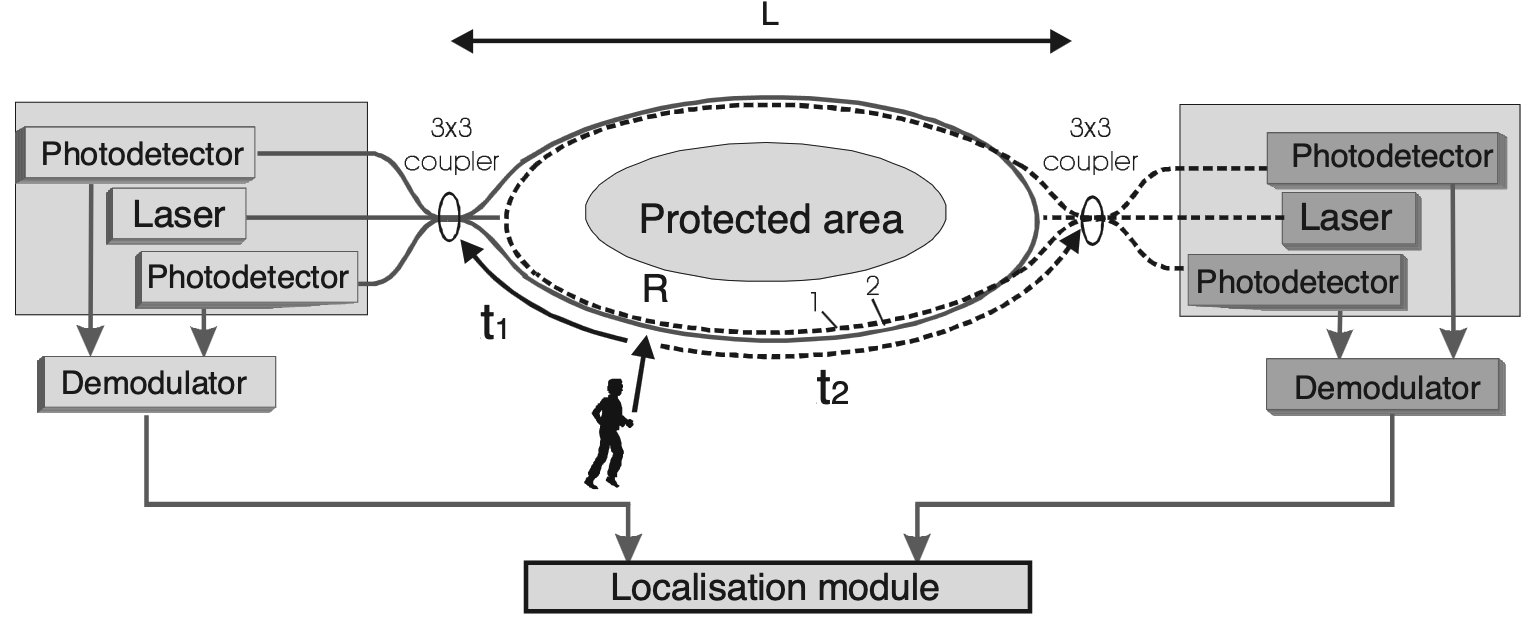
\includegraphics[width=\linewidth]{obrazky/sagnac_interrogator.png}
    \caption{3x3 system for perimeter protection using two Sagnac interferometers~\cite{perimeterpolsko}.}
    \label{fig:sagnac}
\end{figure}

Thanks to research and technological advancements, new devices based on \ac{das} systems are used. These systems use scattering effects that happen in the fiber during the passage of photons through the fiber's medium. These effects are then analyzed at the source of light. The light bounces from imperfections in the fiber and is propagated backward as scattering (\textit{backs-cattering}). Nothing special happens when the fiber is not moving, but when the fiber is affected in any way, for example, by vibrations of an intruder or just by voice alone, the back-scattering changes. These changes can then be analyzed and categorized as an intrusion.


\section{Optical fibers}\label{txt.optical.fibers}


As optical sensing uses existing fiber optic transmission lines, it is important to account for different kinds of optical fibers, materials, and production methods. Optical fibers consist of three main elements \textit{core}, \textit{cladding}, and \textit{coating}. Materials from which core and cladding are made are plastic or glass $Si_2O_3$. 

All-glass fiber dopants, such as $GeO_2$, $P_2O_5$, $B_2O_3$, can be added to all-glass fibers to adjust the refractive index. The core usually has a higher refractive index than cladding by about \qty{1}{\si{\percent}}. Lowering the refractive index can be done by doping fluorine, which is done in the core when the refracting index is too high and needs to be lowered\footnote{https://www.rp-photonics.com/fiber\_core.html}. The radius of core ranges from \qty{3.7}{\si{\micro}\meter} to \qty{200}{\micro\meter} and radius of cladding is up-to \qty{140}{\si{\micro}\meter}~\cite{cabling}.

Plastic optics uses organic material in the form of polymers - chains. Materials used are acrylic, polycarbonate, polystyrene, or liquid silicone. The core of plastic fiber has a popular diameter of \qty{980}{\si{\micro}\meter}.

Although the purpose of the coating is simply protection, the fiber would be very fragile without it. It is usually without special color but can be painted to ease the identification of individual fibers. There are multiple layers of coating, at least primary and secondary. The primary coating is softer to allow the bending of the fiber. Secondary is harder to protect inner layers. Materials such as acrylate, silicone, polyimide,e or carbon are used depending on the application of the optical fiber. for example. For example, acrylate has limited temperature resistance; in this case, silicone is better as it is heat resistant up to \qty{200}{\celsius}\cite{cabling}. For more extreme applications, Polyimide is used as it can withstand temperatures up to \qty{350}{\celsius}, and it is also resistant to chemicals and abrasion~\cite{cabling}.

% \subsection{Fiber modality}\label{txt.optical.fibers.modality}

% Optical fibers can have different kinds of modality depending on manufacturing processes and desired properties of the material. We differentiate multimode and single-mode fiber optic cables. 

% Multimode optical fibers have much larger core diameter compared to the diameter of cladding. This enables 
% %TODO


% Single mode fibers have single propagation mode  per polarization fir a given wavelength. They have very small core diameter, only few micrometers, relative to the cladding diameter. Since they use only single mode there is no inter-modal dispersion\footnote{https://www.rp-photonics.com/single\_mode\_fibers.html}
% %TODO

\section{Light scattering effects in fiber optics}\label{txt.scattering}

Light precisely photons traveling through a medium - atmosphere, glasses, glass optical fiber, or any other medium can bounce from what is called \textit{scattering centers} in the medium. \textit{Scattering centers} are any non-uniformities in the medium such as vacancy defects (missing atoms in otherwise uniform structure), foreign particles, bubbles, trapped gas molecules, fractures, micro-cracks, any changes in refractive index, density fluctuations, manufacturing imperfections, and others~\cite{scatteringcenterbook}. Scattering centers create different kinds of scattering, as will be discussed in the next sections. They include \textit{Mie scattering} (Section~\ref{txt.scattering.mie}), \textit{Rayleigh scattering} (Section~\ref{txt.scattering.ray}), \textit{Raman scattering} (Section~\ref{txt.scattering.ram}) or \textit{Brillouin scattering} (Section~\ref{txt.scattering.bril}). For comparison, Figure~\ref{fig:scattering.comparison} shows all of these different scattering effects:

\begin{itemize}
    \item 1 - input radiation from a laser diode.
    \item 2 - Rayleigh scattering 
    \item 3 and 4 - Brillouin scattering lines %TODO stokes antistokes
    \item 5 and 6 - Raman scattering 
\end{itemize}

\begin{figure}
    \centering
    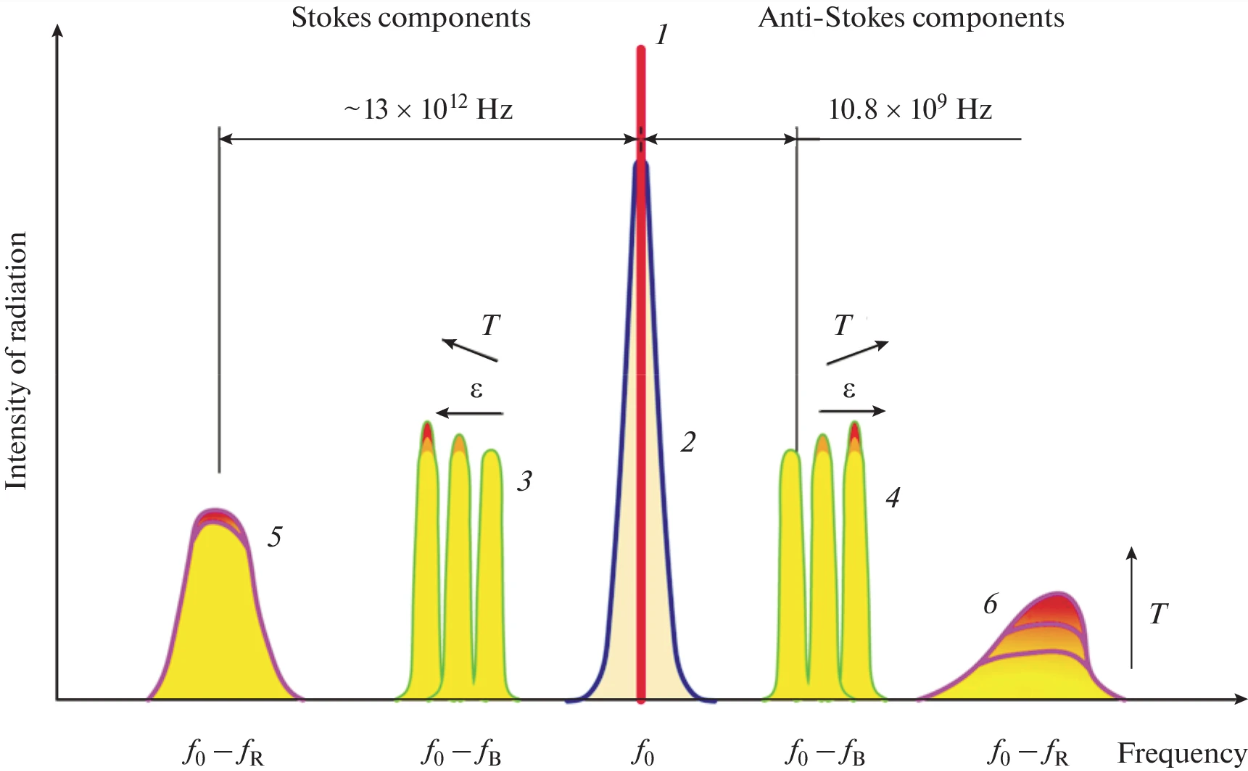
\includegraphics[width=\linewidth]{obrazky/scatterings.png}
    \caption{Comparison of different scattering effects~\cite{scattering.comparison}.}
    \label{fig:scattering.comparison}
\end{figure}

\subsection{Mie scattering}\label{txt.scattering.mie}

\textit{Mie scattering} is an optical phenomenon happening when light traveling through a medium bounces from \textit{scattering centers} the same length or bigger than the wavelength of the light. Mie scattering applies to any spherical particles located in the medium. This also applies to the smaller particles. But we distinguish Mie scattering for particles bigger than the wavelength of light for clarity. For particles smaller than the wavelength of light we distinguish a special case of Mie scattering, and we call it \textit{Rayleigh scattering}, which will be discussed in the next Section~\ref{txt.scattering.ray}. That said, there are differences between these two types. The scattered light's amplitudes are stronger for forward scattering in Mie scattering\footnote{https://www.rp-photonics.com/rayleigh\_scattering.html}. Large defects are usually not uniformly distributed along the fiber, which prevents it from being used in \ac{das} systems~\cite{dasKislov}.

\subsection{Rayleigh scattering}\label{txt.scattering.ray}

Rayleigh scattering is an optical phenomenon named after British physicist Lord Rayleigh. Light is scattered from scattering centers much smaller than the wavelength of the light, for example, individual molecules or atoms. This is opposite to Mie scattering \ref{txt.scattering.mie}, where light is scattering from larger scattering centers. The difference is that amplitudes are the same for forward and backscattering in Rayleigh scattering\footnote{https://www.rp-photonics.com/rayleigh\_scattering.html}. Compared to other scattering processes, Rayleigh is \textit{linear} scattering process whereas \textit{Raman} and \textit{Brillouin} scatterings are \textit{nonlinear}\footnote{Nonlinear light effects occur when the output intensity does not increase proportionally to the input intensity; for example doubling the optical input intensities does not result in double the output intensity. These nonlinear effects tend to weaken significantly at low optical intensities.}.

Only a small portion of the back-scattered light returns to the source - most of it leaves the fiber on the sides. Rayleigh scattering is used in \ac{das}, as discussed in Section~\ref{txt.das}.

When solidified in a medium, not all scattering centers cause Rayleigh scattering. At a wavelength of about 0.95 μm (microns), glass optical fibers have a high attenuation band caused by scattering and absorption by hydroxide ions~\cite{scatteringcenterbook}. Silica glass is an amorphous material with random density fluctuations due to its irregular microscopic structure. This can be limited by an annealing process but can not be removed completely\footnote{https://www.rp-photonics.com/rayleigh\_scattering.html}.




\subsection{Raman scattering}\label{txt.scattering.ram}

The effect photons have when interacting with the crystal lattice of glass is called \textit{Raman scattering}. A transparent optical medium, such as glass, has a crystal lattice. The lattice is naturally vibrating, causing a delayed nonlinear response to the light passing through it. The photon traveling through the medium experiences a loss in energy due to interactions with the medium. This is also called \textit{inelastic scattering}. This is further explained in the next Section~\ref{txt.scattering.bril}.

% The losses happen as vibration energy is exchanged between what are called \textit{phonos}. 

Raman scattering can be measured by sending two light waves with different wavelengths through the optical medium. The  signal with longer wavelength experiences optical amplification at the expense of the one with a shorter wavelength. This is used in Raman lasers, Raman amplifiers, or Raman spectroscopy\footnote{https://www.rp-photonics.com/raman\_scattering.html}.


\subsection{Brillouin scattering}\label{txt.scattering.bril}

Also known as \textit{Mandelsam-Brillouin scattering}, it was first described by Raman in the 1920s. Brillouin scattering is a scattering effect created when light traveling through a medium is scattered during interaction with thermal vibrations of these molecules. As described earlier, it is very similar to Raman scattering. The intensity is much lower than Rayleigh scattering; see Section~\ref{txt.scattering.ray}. But at the same time, much stronger than Raman scattering. For comparison, see Figure~\ref{fig:scattering.comparison}.

The difference between Raman and Brillouin scattering is in the type of interactions with vibrations of the crystal lattice and molecules. To describe the fundamental quanta of lattice vibrations involved in these interactions, we use the term \textit{phonons}. 

There are two types of phonons:

\begin{itemize}
    \item \textit{acoustic phonons} - associated with backward Brillouin scattering; show linear dispersion relation in bulk. 
    \item \textit{optical phonons} - associated with Raman scattering relate to molecular vibrations; have flat dispersion. The forward Brillouin scattering has similar phonon dispersion called Raman-like scattering. 
\end{itemize}

Brillouin scattering in optical fibers primarily occurs in the backward direction, but there can also be some weaker forward Brillouin scattering due to the acoustic waveguide's influence~\cite{bhundred}.

Brillouin scattering is used in Brillouin spectroscopy. Thanks to its uniform distribution along the fiber, it can also be used in \ac{das} systems, although it is much weaker than Rayleigh scattering~\cite{dasKislov}. Brillouin \textit{line width} $\Gamma=1/\tau$ measures material viscosity. In fiber-optic sensing, the Brillouin scattering measures temperature even in distributed manner\footnote{For distributed sensing, please see Chapter \ref{txt.distributed}}~\cite{bhundred}.


\chapter{Distributed Sensing}\label{txt.distributed}

Distributed sensing (in general) is a technology using optical fiber as an array of sensors. It was started in the field of optical reflectometry. There are thousands of virtual sensors along the optical fiber. These sensors are not real devices but rather a clever way of measuring differences in the light signal properties, such as changes in phase. It can measure tension, compression, temperature, vibrations, and other strain impacting the fiber and, consequently, the light passing through it~\cite{dasKislov}. %TODO

Distributed sensing can be based on a single scattering effect (Rayleigh, Raman, or Brillouin). These effects can be combined to improve measurement properties, like accuracy and spatial resolution~\cite{raybril}.

We distinguish multiple distributed sensing systems depending on what is measured:
\begin{itemize}
    \item \emph{Distributed Acoustic Sensing} (DAS) - recording sound and vibrations.
    \item \ac{dvs} - vibration detection.
    \item \ac{dss} - twisting, pulling, bending.
    \item \ac{dts} - temperature measurements.
\end{itemize}

The work will focus on \ac{das} rather than the other Distributed sensing methods because the \ac{das} is used for the measurements. That said, other Distributed sensing methods are quite similar. 

The scattering effects create dispersion effects in the light, which leads to distortion of the light pulse, making it broader. The superposition of neighboring light pulses also limits the transmission frequency. The maximum frequency possible on a transmission line is approximated by Formula \ref{eq:maxfreq}. It takes into account the fact that the light has to travel from the light source to the end of the fiber and back to the starting point at the light source. 

\begin{equation}\label{eq:maxfreq}
    f_i = \frac{c}{n(2L+2P+3D)}
\end{equation}
\bigskip


\section{Distributed sensing based on Brillouin scattering}

Brillouin scattering has been used for distributed sensing since the 1980s when distributed temperature measurement was introduced. Scattering centers for Brillouin scattering are the molecules of the fiber. As they are evenly distributed along the entire length of the optical fiber, it is a perfect candidate for distributed sensing. The Brillouin scattering has a backward and a frontward scattering effect, and both can be used for distributed sensing~\cite{bhundred}.

Brillouin scattering is mostly used for distributed measurements of temperature in \ac{dts} as the scattering effect depends on the temperature vibrations of atoms and molecules in the optic fiber~\cite{distributedrayleigh}.
% \subsection{Backward Brillouin scattering based distributed sensing}

There are also acoustic waves present in the fiber when vibrations or strain affect the fiber. When an acoustic wave interacts with an optical wave, it creates a scattering effect, which produces a new optical wave with a shifted frequency. This wave is referred to as the \textit{Stokes wave} if it has a lower frequency than the original pump wave (the source wave) and as the \textit{anti-Stokes wave} if it has a higher frequency. It is possible to stimulate this phenomenon, resulting in an exponential amplification of the optical Stokes wave. This process is called \ac{sbs}.

\ac{botdr} is a technique based on \textit{spontaneous Brillouin scattering}. Its biggest advantage is that it only needs access to one end of the fiber. Nonetheless, the spatial resolution of this approach is restricted to approximately \qty{1}{\meter}, determined by the phonon lifetime in optical fibers (\qty{10}{ns})~\cite{bhundred}.



%It can be used fully or partially as a complement to the Rayleigh scattering

% It can achieve a spatial resolution of around \qty{100}{\meter} and a measurement range of about \qty{11.57}{km}.

\section{Distributed sensing based on Rayleigh scattering}

Rayleigh scattering, as discussed in Section~\ref{txt.scattering.ray}, is a great candidate for distributed sensing as it can extract three main properties of light - intensity, phase, and polarization. The biggest advantage of Rayleigh scattering is that it is almost completely free from external physical fields - electromagnetic, microwave, and others. The signal is also quite strong power-wise compared to Brillouin and Raman scattering; see Figure~\ref{fig:scattering.comparison} for a comparison of the two. In Rayleigh-based distributed sensors, scattering is used to track and reveal propagation effects such as attenuation and gain, phase interference, and polarization variation. 

Rayleigh scattering originates from the light reflecting back from the molecules and atoms in the fiber. This differs from the scattering from the crystalline lattice (Raman scattering) and atom vibrations (Brillouin scattering). Rayleigh scattering can sense more than strain and temperature - it senses chemical concentration, pressure, vibrations, ionizing radiation, and relative humidity. Polarization enables sensors to detect changes in the magnetic field, twist, and geometrical layout. Detection of phase changes is crucial for sensing based on Rayleigh scattering. 

The back-scattered light can be characterized as the coherent superposition of the light generated from randomly distributed scattering centers in the fiber. The scattering centers create radiation in all directions, but some light travels back to the source, where it can be detected and analyzed. According to Rayleigh's theory, the backscattered light is in phase with the incident light and has the same polarization. The intensity of the light reflected by the scattering center has random quality as the density of the material changes throughout the fiber. Neglecting the polarization effects and dispersion, the complex envelope \textit{b(t)} of the backscattered light can be described as follows in Equation \ref{complexenvelope}. $\beta$ is the propagation constant of the optic fiber, \textit{a(z)} describes the attenuation accumulated up to \textit{z}, \textit{$c_n$} and \textit{$z_n$} are random amplitude and position of the nth scattering center. The \textit{$\tau_n$} is a group delay introduced by the propagation up to \textit{$z_n$}, and factor 2 accounts for the roundtrip propagation; \textit{a(t)} is a wave function of the signal from the light source, the statistics of \textit{$c_n$} and \textit{$z_n$} are not important in this context~\cite{distributedrayleigh}.


\begin{equation}\label{complexenvelope}
    b(t) = \sum c_n e^{-2[\alpha(z_n)+j\beta z_n]} a(t-2\tau_n)
\end{equation}
     
\begin{equation}
    \tau_n = z_{nd} \beta / d\omega
\end{equation}

The measurement involves retrieving the attenuation \textit{$a(z)$} by measuring \textit{$b(t)$}. This creates two modes of measurement either it means to first probe the fiber by continuous wave signals at different frequencies to measure the frequency response and then compare it to the values during the real measurement (frequency domain), or to measure the response of the fiber by analyzing the roundtrip propagation through the fiber (time domain)~\cite{distributedrayleigh}.


%TODO pokracovat timedomain, pokracovat frequency domain a DOFS


\section{Optical reflectometry}\label{txt.reflectometry}

Optical reflectometry is used for measuring optical cable properties; it can detect defects, joints, breaks, or other damage and their location on the wire. It is the basis for \ac{generalotdr} or \ac{ofdr} and other optical sensors such as \ac{das}. A~pulse of light is sent from the source, such as a light-emitting diode (LED) or a laser diode (LD). The light travels from the source through the optical fiber in pulses and is reflected from the other side of the wire through connections, breaks, damage, or imperfections in the material. All of these create some back-scattering toward the light source~\cite{progress}. 






\subsection{Optical Time Domain Reflectometry}\label{txt.reflectometry.otdr}

\ac{otdr} is the most widely used method. When a strain is applied to the fiber, it causes phase-shift changes in the light signal. Provides high sensitivity, resolution, and sampling rates in the frequency range between hertz and kilohertz. \ac{otdr} has limitations in measuring slowly changing effects and noise components~\cite{distributedvibrsensingotdr}. The optical time domain reflectometer was proposed back in 1976 by Barnoski and Jensen. The principle is to send a light pulse through the fiber to measure the impulse response; see Figure~\ref{fig:simpleotdr}.

\begin{figure}
    \centering
    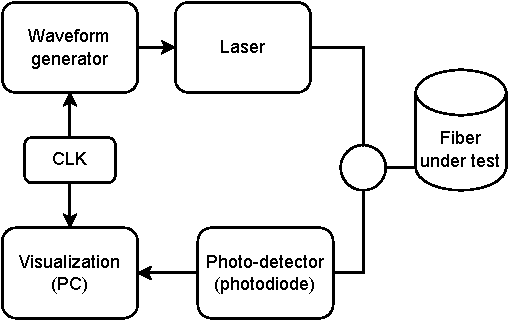
\includegraphics{pdf/optic_reflectometer.drawio.pdf}
    \caption{Example of basic OTDR reflectometer.}
    \label{fig:simpleotdr}
\end{figure}

% The goal is to use very precise light pulses with specific wavelengths, and we also  want them to be as short as possible. Unnecessarily long pulses lower the maximum pulse frequency as shown in the relation \ref{}


% \subsection{(\acs{otdr})}   %\acl{otdr} \label{txt.reflectometry.otdr2}


% %TODO
% https://www.flukenetworks.com/expertise/learn-about/otdr

% as shown in Figure~\ref{fig:otdr.diagram}.

% \cite{otdr.advances}

% \begin{figure}
%     \centering
%     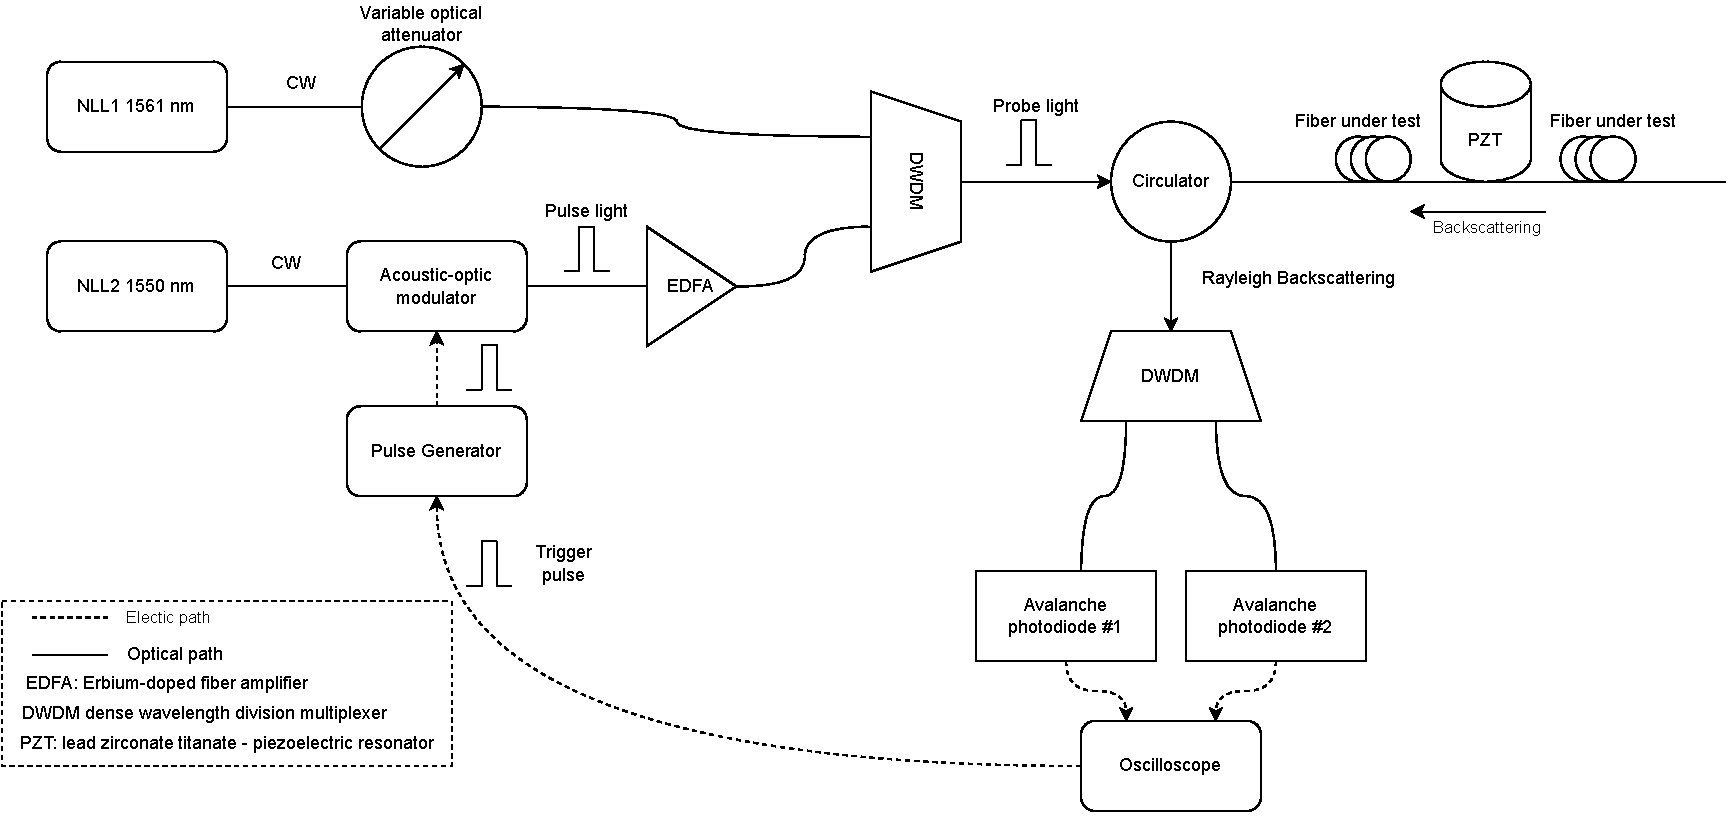
\includegraphics[width=1.5\linewidth, angle=90]{pdf/otdr.diagram.drawio.pdf}
%     \caption{Example of \ac{otdr} measuring system.}
%     \label{fig:otdr.diagram}
% \end{figure}

\subsection{OFDR}\label{txt.reflectometry.ofdr}

\ac{ofdr} analyzes interference of signal between the initial signal and the back-scattered signal but focuses on the frequency scan. A~source of light has to be a laser diode that can be precisely tuned to a certain frequency. The signal given by \ac{ofdr} contains frequency information that can be processed with the Fourier transformation. The output would be the position of the reflective elements along the fiber length. There are also other methods to measure light properties such as \textit{C-OFDR} - coherent version of OFDR using light with the frequency with linear dependency but having problems with high noise levels, and \ac{dss} - Mandelstam-Brillouin~\cite{kislov_das_newparadigm}.






























\newpage
\section{Distributed Acoustic Sensing}\label{txt.das}

Implementation of \ac{das} system is usually done by \ac{generalotdr}, \ac{ofdr}, or analysis of other light properties such as polarization and back-scatter correlation. \ac{das} allows the measurement on thousands of points on an optical wire without the need to cut the wire or have multiple sensors distributed along the wire. The measurement mechanism is based on optical reflectometry, the same as in \ac{dts}, a variant of \ac{generalotdr}. \ac{das} relies on non-uniformities spread evenly along the fiber. As discussed in Section~\ref{txt.scattering.ray}, the best suited for this application is Rayleigh scattering, which describes light scattering from particles smaller than the wavelength of the light. In this case, the particles are molecules and atoms in the fiber.

Scattering effects suitable for the use in \ac{das} measurements are Brillouin, Raman and Rayleigh 

During measurement, pulses of light are sent into the optical fiber. The fiber creates a light scattering (e.g., Rayleigh scattering) in the glass that travels back to the sensing unit (on the same side as the light source), which can be interpreted based on the arrival time as a position on the wire. Back-scattering light from the optical fiber segment is detected at the light source. If a strain or a vibration is applied to the optical fiber, it detects changes in amplitude or phase, which means that the fiber wire segment is externally affected somehow. \ac{das} is used in a wide range of applications, from locating seismic activity, locating trains along the train tracks, as a~gyroscope or an accelerometer or even as a~microphone~\cite{WangYu2017RDVM},~\cite{kislov_das_newparadigm}.

\ac{das} uses optical fiber as many sensors along its length. The fiber is capable of detecting vibrations along it can also detect acoustic properties as they are also vibrations but of sound. These sensors allow for measuring acoustic properties such as frequency, amplitude, and phase~\cite{WangYu2017RDVM}. 

When installing cables, it is crucial to consider both cable design and installation methods. The rigidity of the fiber is a significant factor because stiffer cables can reduce sensitivity. Optimal results are achieved by utilizing a single-mode fiber with minimal protection buried in the ground. The contact with the surroundings is also essential as it can impact the signal-to-noise ratio and alter the frequency content of the recorded signal.

When using an existing fiber optic infrastructure, it is hard to know what parts of the fiber are in contact with, for example, soil or ground, when measuring seismic activity, as good contact is crucial to yield good results. When monitoring boreholes, the wire can be lowered into the hole, but the quality of measurements will vary. For this purpose, mounting the cable to the bore pipe is a better solution. Good contact with the ground or seafloor is very hard to achieve, for example, in underwater applications for measuring underwater seismic activity. When laying the fiber optic cable, the cable can stretch over crevices and underwater valleys and dips, failing to make contact, which hinders the measurements and has to be accounted for.

There are also special optic fibers being developed for making the connection with the ground uniform. They have a better signal-to-noise ratio and good transmission of external vibrations on the fiber while maintaining mechanical protection~\cite{dasKislov}.

\subsection{Measurements}

The fiber is divided into segments representing a sensor located along the fiber. These sensors are just virtual - they are not real devices. By measuring time differences between the time light was transmitted and the reflected light reached the sensor, interrogator devices can identify what portion of the fiber is affected. Each segment is called \textit{Gauge Length} and represents a sensor. The location of a sensor is in the middle of the gauge length. Sometimes neighboring segments can overlap. The signal is formed between two points on the reflectogram corresponding to the edges of the gauge length. Setting gauge length is crucial to get the correct measurement. If the gauge length is too small, it degrades the signal-to-noise ratio. If too big, it creates signal distortion. Calibration is sometimes necessary to account for insufficient ground contact and to make measurements as precise as possible~\cite{dasKislov}. 

\subsection{Advantages of DAS systems}

The possibility of using existing fiber-optic infrastructure makes deploying sensing arrays very easy and cheap. Unused fiber optic wires laid for later activation, when higher bandwidth is required, are called \textit{dark-fibers} and can also be used for distributed sensing. \ac{das} technology can be applied to many different applications with the biggest advantages over the traditional sensors and electric devices in terms of no electromagnetic interference and adverse conditions - radioactivity, harsh chemical environments, high temperature, underwater, and others, see Section~\ref{txt.sensing.usage}. It is hard to imagine the limitations of this new technology~\cite{dasKislov}.

\subsection{Disadvantages to traditional sensors}

When using \ac{das} for seismology, good contact with the ground is necessary. With insufficient contact, the \ac{das} technology can provide unsuitable values. Traditional seismometers plot data instantaneously in comparison to \ac{das} systems that plot data with time delay~\cite{dasKislov}. The size of fiber-optic sensors such as fiber-optic gyroscopes is still huge compared to \ac{mems} sensors used in today's microelectronics. \ac{mems} can be soldered to PCBs and used in a wide range of applications, but they also have weaknesses, like poorer precision and low heat resistance. 

\subsection{iDAS}\label{txt.idas}

The distributed acoustic sensor is a~new addition to distributed optical fiber sensors used in the energy industry and can be used in many applications, for example, in detecting seismic activity. iDAS (intelligent distributed acoustic sensor) is one type of DAS sensor. One of the applications of this sensor is to record an acoustic signal. To determine the signal fidelity, a certain part of the wire is subjected to a known signal, for example, a sine wave. A measurement is made, and the result is compared with the existing recording device. The result suggests that iDAS has very good signal properties. The measured signal shows that almost no measurable crosstalk is exhibited between the two sensing channels on the wire.

The maximum sampling rate can be calculated from the speed of light that travels in glass at a speed of about \qty{200000}{\km/\s}, which corresponds to approximately \qty{10}{\kHz} for \qty{10}{\km} long wire~\cite{WangYu2017RDVM}.

% 10 kHz == 10 km, 1 kHz == 100 km [doplnit vzorcek]

\begin{itemize}
    \item Acoustic bandwidth.
    \item Dynamic range - \qty{120}{\dB} as reported in~\cite{dasseismic}.
    \item Spatial resolution - about \qty{1}{\m} to \qty{10}{\m}, but up to \qty{25}{\cm} is possible.
    \item Measurement range - The fiber length can be anywhere from a few hundred meters to more than \qty{100}{\km}.
\end{itemize}


\section{OptaSense ODH-F}\label{txt.optasense}

Data used in this project are obtained from \textit{OptaSense ODH-F Distributed Acoustic Sensing Interrogator}\footnote{\url{https://www.optasense.com/technology/odhf/}}(Interrogator). This device is capable of monitoring optical fiber up to \qty{50}{\km} long (in qualitative mode). It allows for sequential monitoring of four cables at the same time. It is used for in-well flow monitoring, pipeline integrity management, and border security. 

OptaSense uses \ac{cotdr}, for further explanation see Section~\ref{txt.reflectometry.otdr}

% TODO

OptaSense comes with \textit{DxS Visualization Software} capable of analyzing and processing output data from the unit. It can show the signal spectrum in a waterfall graph and create analysis, process the signal using \ac{fft}, and extract data to \verb|.wav| format. It has the limitation that it can only run in the Windows ecosystem and is proprietary software, so scientists cannot change how they work with the data or how it is displayed.

\section{Existing technology for HDF5 data visualization}\label{txt.design.existing}

This section focuses on data processing and visualization using existing software for visualizing scientific data. First is OptaSense OS6 software which is a purpose-made solution for OptaSense devices. Next is the h5web library, written in React, which creates a web page for visualizing the content of HDF5 files.



\subsection{HDF5 file format}\label{txt.hdf5}

The data captured by the Optasense Interrogator is collected in \ac{hdf} and saved into a file with \textit{.h5} suffix. \ac{hdf} creates a model for managing and storing data. The HDF Group\footnote{\url{https://www.hdfgroup.org/}} maintains the format and its corresponding software package. Specifically, the \ac{hdf} format is used to store data, but only one of the three parts makes up the full \ac{hdf} model. Parts of the \ac{hdf} model are:

\begin{itemize}
    \item File format - files ending with .h5
    \item Data model - specifies the building blocks of the \ac{hdf} file format
    \item Software - libraries, tools, APIs
\end{itemize}

\bigskip

\ac{hdf} data model has a folder-like organization, where the folders are called \textit{groups}. This model specifies the format in which the data are stored in the form of \ac{adm}, which specifies the organization of the data and the types of data. Every \ac{hdf} file has to have a~root group \textit{``/''}. Working with groups is very similar to directories on Linux systems; see Section~\ref{dir:filestructure}. Each group can have \textit{datasets} that contain raw data, attributes, data types, and other objects. \ac{hdf} file can also specify links to other libraries and tools such as compression and filtering.

\bigskip
\ac{hdf} dataset has connections with other HDF5 objects:

\begin{itemize}
    \item \textbf{attributes} - named data object containing the name and the value
    \item \textbf{datatypes}:
    \begin{itemize}
        \item Atomic datatypes - time, string, integer, float.
        \item Composite datatypes - array, enumeration, compound, variable length.
    \end{itemize}
    \item \textbf{data} - data itself, for example, the result of measurement.
    \item \textbf{dataspace} - the shape of the data.
\end{itemize}


\begin{figure}
    \centering
    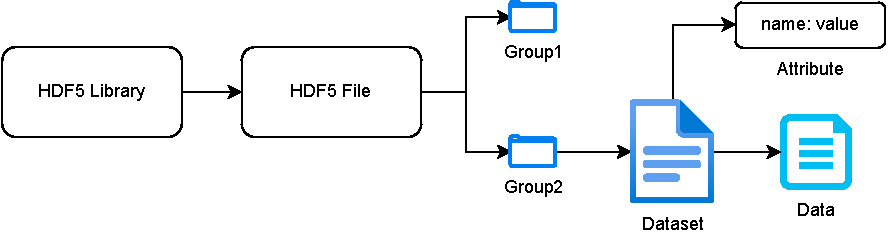
\includegraphics[width=\linewidth]{pdf/hdf5_file_structure.pdf}
    \caption{Basic HDF5 file structure.}
    \label{fig:filestructure}
\end{figure}

% \newpage


\subsection{OptaSense OS6}\label{txt.design.optasense}

The OptaSense company provides visualization software for their devices called OptaSense OS6\footnote{\url{https://www.optasense.com/technology/os/}}. It supports only Windows operating system. OS6 provides features for monitoring areas or land, for example, a compound or an industrial building. This product is tailor-made for OptaSense devices by the OptaSense company. This system has only one window for everything. The primary view is the monitored area; the background picture is the aerial view of the monitored space, as seen in the picture \ref{fig:ossix}. The user can open the sidebar on the right side. The sidebar provides multiple different options:

\begin{itemize}
    \item \textbf{Spectrogram} - Raw data visualization.
    \item \textbf{Alerts} - When an action is detected along the wire, it is logged.
    \item \textbf{Notifications} -  Notifications about system state.
    \item \textbf{System status} - Overview of all OptaSense units and their state.
\end{itemize}

There is also a feature that takes raw data from interrogator units and processes them using machine learning. This way, different actions are detected and categorized into different alerts, such as walking, driving cars, etc. In addition, the user can see the activities detected and triggered in the area overview with live monitoring and a timeline at the top of the screen. To easily look at different locations or start a new view, a feature \textit{type to search} lets the user start a search by typing into the view. For example, the user starts writing ``water...'' as a waterfall, and the program will look for this feature and open the waterfall visualization window. OS6 saves all detected activities, shown in the \textit{Historic timeline} window, which shows all alerts during a specified time range. The animations look very nice, although some look choppy, mostly when showing activities on top of the waterfall view. 

It proves that it is possible to create a real-time data visualization from the \ac{das} system. It lacks one important step, which is the ability to be used not only on Windows machines and be multi-platform. And although it provides enough tools for data analysis, it is unsuitable for further scientific work such as custom editing the visualization or exporting data to images and further processing for machine learning and activity categorization.

\begin{figure}[t]
    \centering
    \includegraphics[width=\linewidth]{obrazky/OSsix.png}
    \caption{OptaSense OS6 visualization software~\cite{ytossix}.}
    \label{fig:ossix}
\end{figure}


\subsection{h5web}\label{txt.design.h5web}

The \verb|h5web|\footnote{\url{https://h5web.panosc.eu/}} library is a set of components written in React\footnote{React is a JavaScript library used to create interactive user interface \url{https://reactjs.org/}}. H5web uses existing HDF5 libraries, such as h5wasm (reading HDF5 files in the browser) and h5grove (server for accessing HDF5 files). It displays the contents of the HDF5 file and shows different graphs according to the input from the user. From the presentation of the library by its developer, it is safe to say that although it provides the necessary equipment for opening HDF5 files elegantly and provides advanced graphing techniques, it lacks the ability to receive the data and display them as they were coming from the \ac{das} system. For this purpose, the library would need to add support by creating a new React component capable of such behavior.

\begin{figure}
    \centering
    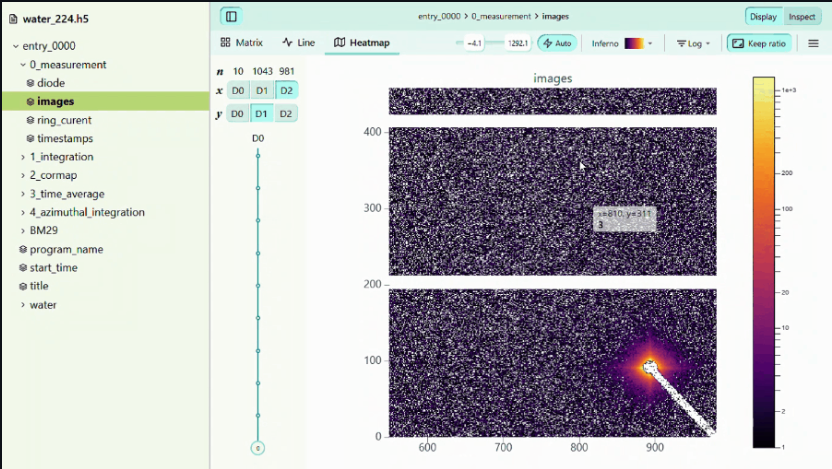
\includegraphics[width=\linewidth]{obrazky/h5web.png}
    \caption{h5web application with an example data visualization.}
    \label{fig:h5web}
\end{figure}

\newpage


\chapter{Software design}\label{txt.design.design}

There are many ways to implement data visualization. Still, choosing the right solution, programming language, or framework is hard, so this chapter first provides information on what this application should do. Second, it studies the existing OptaSense software and other solutions accessible from the internet. Lastly, it explains the software design decisions for implementing this data visualization.

% \section{Software design}\label{txt.design.sw}
\subsection{Usecases}\label{lab:usecases}\label{txt.design.sw.usecase}

The task is to fulfill the usage requirements, as seen in the use case figure \ref{fig:usecase}. Users need to see and view what is happening in their perimeter on their screen. For this purpose, the best data visualization is a waterfall graph, similar to a spectrogram, displayed as the main element. It should have an editable color map to adjust the sensitivity. The waterfall view should be an animated waterfall graph and ideally display real-time data on the screen, similar to the OS6 system; see Section \ref{fig:ossix}. In addition, the user should perform selection and zoom on the waterfall graph. The user should be able to edit properties of the graph, like changing the data range and choosing the channels he or she wants to see. The user should be able to export the data to a WAV file by clicking a button and then viewing and playing the audio file. There should also be a waveform display available to show the playing data.

\begin{figure}[h]
    \centering
    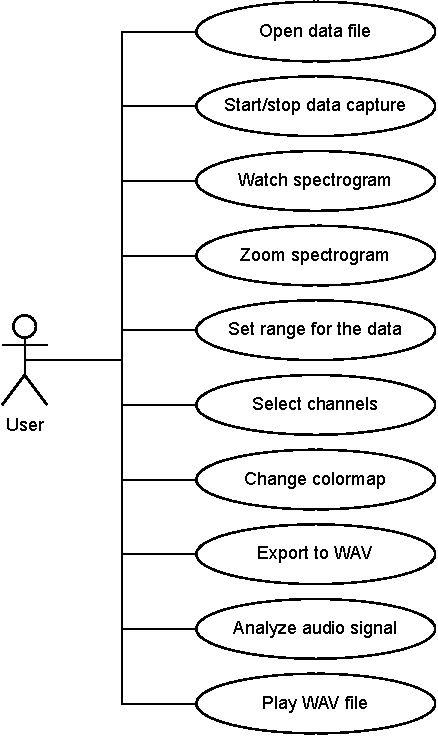
\includegraphics{pdf/usecase.drawio.pdf}
    \caption{Application usecases}
    \label{fig:usecase}
\end{figure}

\subsection{Application requirements}\label{txt.design.sw.requirements}

From the use-cases in Section \ref{lab:usecases}, it is understandable that the application should have certain features. Apart from the given use cases, there are other important requirements:

\begin{itemize}
    % \item Support for real-time data plotting - graph updates or animation; fetching the data online from the OptaSense Interrogator and displaying it in real-time
    \item Multiplatform - the application should run on any device and still support all features
    \item Data processing - subsampling data to save data throughput
    \item Plot editing and animation - changing plot properties
    \item Reading offline data - possibility to read local files or upload files into the application
    % \item 
\end{itemize}

% There is the option to create an application running on the operating system

\begin{figure}[h]
    \centering
    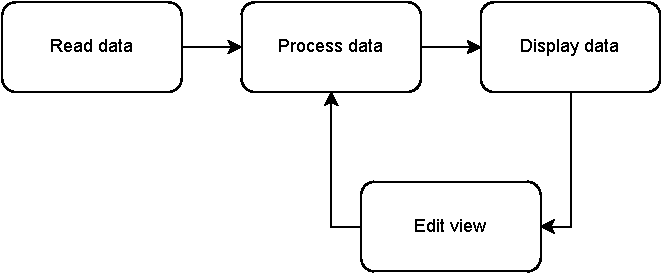
\includegraphics{pdf/simple_application.drawio.pdf}
    \caption{Data flow in the application - reading the data then processing the data and displaying it (optionally) edit the view}
    \label{fig:dataflow}
\end{figure}

It is necessary to choose the right programming tools to satisfy all features. The right way to find the right solution in programming is to \textit{divide and conquer}. This means finding all the pieces that will make the application. First, there must be an idea of what will happen with the data. Firstly, it has to be read, processed, and then displayed. The optional step is to edit the data or change the view; this data flow can be seen in Figure \ref{fig:dataflow}. 

% Multiplatform requirement removes many options - like creating a simple GUI application, as creating a multiplatform high-performance application is quite a feat and is beyond this project. So the result is making a web site and display  there is one solution either using 

From the data flow application, an overview can be made for a web application, as seen in Figure \ref{fig:app_overview}. The overview illustrates what parts the application will have. The back-end or server application will be responsible for reading HDF5 files and processing data. It will provide some interface or API for the client application to fetch\footnote{\url{https://developer.mozilla.org/en-US/docs/Web/API/Fetch\_API}} the data. On the client side, the client has to be able to create visualizations of the data and provide a user interface to change application properties.

\begin{figure}
    \centering
    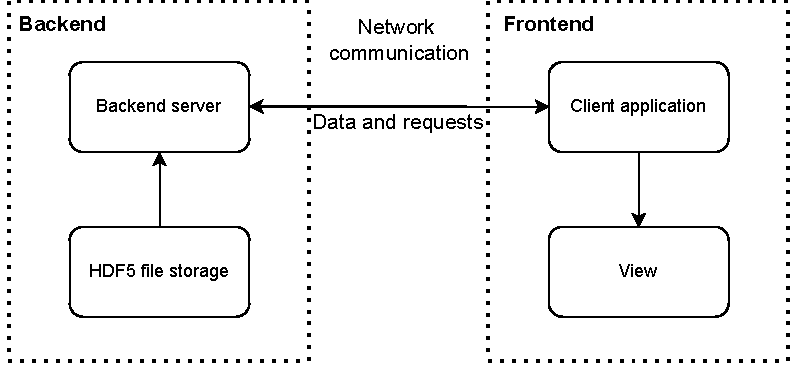
\includegraphics{pdf/appstack_general.drawio.pdf}
    \caption{Application overview. The server reads the data from the data storage and sends it to the client application, where it is shown to the user}
    \label{fig:app_overview}
\end{figure}


\section{Back-end}\label{txt.design.backend}

The purpose of the back-end part of the application is to read, process, and send the data to the client part of the application, as seen in Figure \ref{fig:app_overview}. Reading the HDF5 data is done as explained in Section \ref{txt.implementation.reading}.


\subsection{Existing REST based servers for HDF5 data access}\label{txt.design.rest}

There is a wide range of REST server implementations; HDF Group provides documentation for its RESTful API\footnote{\url{https://support.hdfgroup.org/pubs/papers/RESTful\_HDF5.pdf}}. They have prepared a few RESTful server implementations for their data format. There are many more implementations of REST servers, such as the Python Simple HTTP server. Here is a list of some possible implementations \cite{hdfrest}:

\begin{itemize}
    \item \emph{h5serv} - REST-based service to access HDF5 data written in Python (HDF5 Group).
    \item \emph{HSDS} (Highly Scalable Data Service)\footnote{\url{https://github.com/HDFGroup/hsds}} - Python implementation of the REST-based service to access HDF5 data stores. Data can be stored in the POSIX file system or object-based storage such as AWS S3. It can run in a Docker as a single machine or on a Kubernetes cluster.
    \item \emph{hdf-rest-api}\footnote{https://github.com/HDFGroup/hdf-rest-api} - is HDF5 REST API that provides CRUD support (create, read, update, and delete) for all HDF5 objects.
    \item \emph{h5grove} - Back-end service written in Python providing access to HDF5 file content.
    \item \emph{http.server} - Python implementation of a simple HTTP server. However, this is better used only for testing purposes when accessing local files.
\end{itemize}


\subsection{WebSockets}\label{txt.design.websocket}

WebSockets (or WebSocket API) enable two-way communication over \ac{tcp}. IEFT standardized it in RFC6455\footnote{https://www.rfc-editor.org/rfc/rfc6455}. All modern browsers support the WebSocket protocol.

The communication starts with an HTTP-compatible handshake, so only one socket can communicate with the server. There are also other header types available for different uses. The server responds with an HTTP Upgrade, the connection is established, and bidirectional communication can begin. Communication closes when either side decides to close the connection and starts closing the handshake. The other side responds with a \textit{Close frame} message, closing the connection. 

The protocol is frame-based, as is HTTP protocol, but simultaneously, it tries to be frame-based as little as possible. Just enough to make sure that it can use the HTTP interface for communication; otherwise, it tries to be as minimalist. The authors of the WebSocket protocol wanted it to be low-level, and as close to TCP as possible \cite{websock}. WebSockets have an implementation in the Python programming language called \verb|websockets|\footnote{https://pypi.org/project/websockets/}.

\begin{figure}[h]
    \centering
    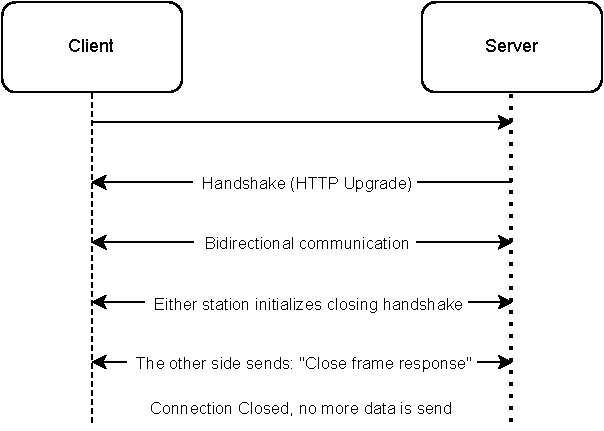
\includegraphics{pdf/websocket.drawio.pdf}
    \caption{WebSocket handshake, communication, and connection close diagram.}
    \label{fig:websocket}
\end{figure}


% \subsubsection{Processing data}\label{txt.design.datapprocessing}
% TODO???

\section{Frontend}\label{txt.design.frontend}
% \subsubsection{WebGL}\label{txt.design.frontend.webgl}
\section{Svelte}\label{txt.design.frontend.svelte}

Svelte is a component framework written in JavaScript, using a new approach to building web applications. Instead of looking for differences in virtual DOMs as React does, which is done in the browser and consumes quite a lot of resources, Svelte does everything at the compilation stage. The compilation output is a JavaScript file \verb|bundle.js|, which contains all the necessary code to run the web application or, better said, it manipulates the DOM directly. The result is a fast and reactive web page, it also saves resources, and the code can be run on small devices like handheld devices. Web development is also very enjoyable because compilation does not take long, and the changes can be visible immediately. The structure of a Svelte component consists of three parts - JavaScript code tag \verb|<script>| a style tag \verb|<style>| and other HTML elements. 

Svelte does not provide more advanced features like page routing. For this purpose, the Svelte team created SvelteKit, which is a~framework for building web applications and allows page routing. Routing is folder-based - the developer creates a folder and file structure.

\begin{verbatim}
src/routes/about/+page.svelte <=> /about
src/routes/about.svelte <=> /about
\end{verbatim}

Svelte has been changing and has become a Vite \footnote{\url{https://vitejs.dev}} plugin. Vite provides fast development experience by running a development server, in the case of Svelte - Hot Module Replacement (HMR)\footnote{\url{https://vitejs.dev/guide/features.html\#hot-module-replacement}}. This way, every change made during development can be immediately seen in the browser without reloading the page, which makes development much faster and more enjoyable. It is necessary to say that Svelte is still in development, and although it is now at version 3, it is possible that it will change in the future. 

When fetching the data from the server, it is good practice to move this functionality to a Svelte Store. From a programming point of view, a store is an object with a \verb|subscribe()| function. An example of a WebSocket implementation in Svelte can be the Svelte component library \textit{svelte-websocket-store}\footnote{\url{https://github.com/arlac77/svelte-websocket-store}}.


\subsection{Real-time capabilities}\label{txt.design.frontend.realtime}

The data bandwidth (the amount of data necessary to be sent from the server side to the client side) of the application is the biggest factor. The OptaSense Interrogator can produce quite a lot of data, but if it is saved in an HDF5 file, as it is compressed, it is quite small. As discussed in Section \ref{txt.implementation.reading}, a \qty{10}{\second} file produces around \qty{52}{MB} of data. When this data is transformed into text form, it has only \qty{420}{MB}, and when transformed into JSON, it has \qty{946}{MB} as the data are read at  \qty{10}{kSPS}\footnote{\ac{sps}}. Data will be displayed on display with standard resolution and cannot display \qty{10000}{\ac{sps}} on a small part of the display. Data processing is necessary for this purpose. 


% \subsubsection{Data processing}\label{txt.design.frontend.dataproc}

% Data processing can be done on the server or browser. As the browser will be busy redrawing waterfall visualization, it is better to preprocess data on the server side. Server-side preprocessing will also save bandwidth as the data will be significantly filtered. 

% Sending data in the form of REST requests and responses can be possible, but it is really useful only when sending a small HDF5 file as a whole, not as a stream of data, and although the h5grove backend provides the ability to read sections of the data set for  The respective bandwidth would be \qty{}{}

 % The JSON file is quite large - the original HDF5 file is only \qty{52,7}{MB} and the JSON file is \qty{946,6}{MB}. The dump text file is half the size and provides the same information, but the datasets are harder to understand, but the whole file is only half the size of the JSON file at ``only'' \qty{420}{MB}. The JSON format is much easier to read. The structure of the file is divided into three parts:


% %TODO


\subsection{Software design frontend for DAS data visualization}\label{txt.design.frontend.dataviz}

As we discussed in Section \ref{txt.design.optasense}, it is possible to create such software to display the data in real-time. The proprietary application from Optasense is a native Windows application. The requirement for this application was to be able to run on multiple platforms. The chosen platform is the Python back-end for opening files, processing the data, and sending the data to the client application using Svelte. The backend will process the data as explained in \ref{txt.design.datapprocessing}. The waterfall graph will be an HTML Canvas element that displays the data in real-time, redrawing itself as the data arrive at the browser. For ease of displaying the data in Canvas, D3.js will be used. D3 will, for example, apply a color map to the correct scale according to the data. The user interface written in Svelte will also have inputs to change the properties of the visualization so that the user can select specific channels from the data, choose subsampling effect properties, cutting the frequency range. The ability to export the data to a WAV file will also be implemented the same way as done in Section \ref{lab:hdftowav}.

\begin{figure}
    \centering
    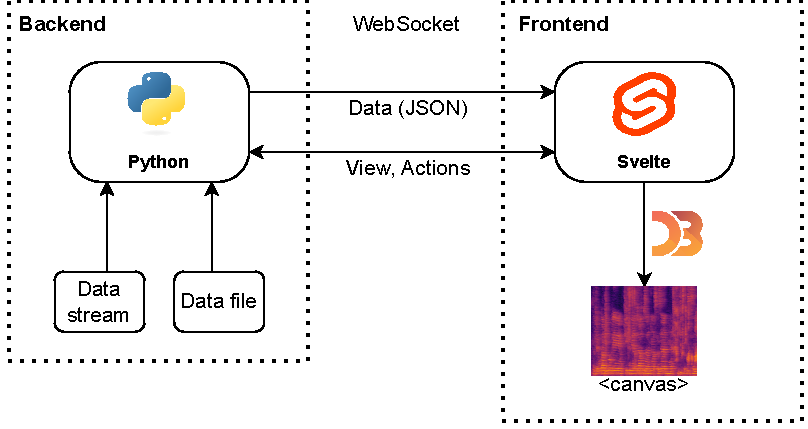
\includegraphics{obrazky/appstack.drawio.pdf}
    \caption{Application overview}
    \label{fig:app_overview}
\end{figure}







\section{HTML chart rendering}

For in-browser rendering, two main options exist using HTML canvas rendering or using \ac{svg} elements. In this section, we will discuss both their advantages over each other and their drawbacks. In general, Canvas rendering performs better than \ac{svg} rendering. This is because SVG is based on a \ac{dom} structure\footnote{text-based structure defining objects displayed on the web page. https://developer.mozilla.org/en-US/docs/Web/API/Document\_Object\_Model/Introduction}. It is more suitable for large datasets and graphics-heavy games and animations\footnote{https://www.chartjs.org/docs/latest/\#canvas-rendering}.

\subsection{HTML SVG graphics}

\ac{svg} is an XML-based markup language developed by W3C\footnote{World Wide Web Consortium www.w3.org}. It describes 2D vector graphics in XML text files. SVG supports three types of graphic objects: vector shapes, bitmap images, and text. The main advantage compared to bitmap graphics is that all the elements can be rendered at any size without losing quality. 

The description of graphics elements is the same way as the web page description written in HTML to the final web page. There are tags for different geometrical objects, for example, rectangles, ellipses, lines, and animations. Everything is defined in an XML text file which can be edited, searched, or compressed\footnote{https://developer.mozilla.org/en-US/docs/Web/SVG}.

Data visualization using \ac{svg} graphics results in smooth and sharp visualizations. It also enables interactivity with each displayed object - selecting, hovering, or zooming. Libraries for \ac{svg} manipulation manipulate text based on the data given. \ac{dthree} is a JavaScript library using HTML, SVG, and CSS to visualize data. It can bind data to the HTML DOM and then apply data-driven transformations. \ac{dthree} allows developers to create custom visualizations as it is not a charting library but a set of data visualization tools. It is also the base for other charting libraries that build on the \ac{dthree}'f framework. They include Plotly's JavaScript implementation, C3.js\footnote{https://c3js.org/} or Britecharts\footnote{https://britecharts.github.io/britecharts/}.

\subsection{Canvas graphics}

JavaScript makes drawing to the HTML \verb|<canvas>| element possible with the use of \textit{Canvas API} or \textit{WebGL API}. It can render data visualizations, game graphics, real-time video processing, and animation. WebGL can draw 2D and 3D graphics to the canvas element, but we will not be covering WebGL further. Canvas API focuses on 2D graphics. Libraries using Canvas API that make rendering to canvas easier differ on the use case - EaselJS (web game development), Konva.js (desktop and mobile applications), Chart.js, and many more. Canvas rendering depends on the resolution of the screen. 

\verb|<canvas>| tag is used for drawing graphics. You can imagine the canvas as a rectangular area with the starting point at the top left corner with coordinates (0,0) and defined width and height. By default, this area is transparent. When we want to draw to it we need to call functions from the Canvas API. They define basic shapes and primitives that can be drawn on the canvas. Rectangles and paths are the only primitive shapes that can be drawn to \verb|<canvas>| element, and more complex shapes can be drawn by combining these primitives\footnote{https://developer.mozilla.org/en-US/docs/Web/API/Canvas\_API/Tutorial/Drawing\_shapes}. Basic example of drawing to canvas can be seen in the code snippet \ref{lst:canvas.example}. Usually, the functions define certain shapes filled with color and added to the canvas. Then "clearing" functions remove what is displayed or create transparent areas. Lastly, there are "stroke" functions that create lines. 

\begin{lstlisting}[frame=single,numbers=right,caption={An example implementation of drawing to canvas.},label=lst:canvas.example,basicstyle=\ttfamily\small, keywordstyle=\color{black}\bfseries\underbar,]
function draw() {
    //First, we need a reference to canvas element
    const canvas = document.getElementById("canvas");

    //Next, we need context to draw to
    const ctx = canvas.getContext("2d");

    /**** Drawing  ****/
    
    // drawing a rectangle to canvas
    ctx.fillRect(10, 10, 100, 100);
}
\end{lstlisting}

The biggest drawback of displaying data with \verb|<canvas>| is its lack of interactivity with displayed elements and poor text rendering capabilities\footnote{https://www.w3schools.com/html/html5\_svg.asp}. The interactions are achievable but usually require "hacky" solutions like hidden canvas or invisible layers. Having more than 1000 objects rendered on screen that can be selected can also cause performance issues. 


\subsubsection{Drawing to canvas and animation}

Creating animations on canvas elements is done in two ways. Calling function \verb|setInterval()| in which a callback function is given with a time delay value in milliseconds. This was a preferred way to create animations until the implementation of the \verb|requestAnimationFrame()| method. It also takes a callback but without a time value. This is because it just tells the browser to perform an animation, so the developer doe not need to worry about managing the number of frames per second. It can perform a redraw up to the frame rate of the screen. So if the user has a \qty{60}{Hz} screen, it redraws every \qty{16.6}{ms} and respectively, if \qty{120}{Hz} screen, it redraws every \qty{8.3}{ms}. For updating at a lower FPS than the screen refresh rate, the callback is passed with a time stamp value of the request. This value can be compared with the time of the previous update, and if the delta is smaller than desired, it will not update the canvas. If the delta is bigger, it will allow the redraw.

\subsection{Heatmap visualization}\label{txt.design.frontend.heatmap}

A \textit{heatmap} is a graph depicting data values in cells in a two dimension grid. Usually, the cell shape is made of simple rectangles or squares, but any shape is possible. For example, population data can be visualized on a map or a globe. The color of each cell is a representation of the value. Choosing the right color palette; otherwise, the data can be hard to understand. We discuss color palettes in Section \ref{txt.design.frontend.colormap}. The colors used in the heatmap indicate the relative values of the data. Depending on the color palette chosen, the result can be a visualization with darker colors representing higher values and lighter colors representing lower values. Showing a color scale legend near the graph is good practice for more straightforward data interpretation.

Heatmaps are used in different scenarios as they can make data more interesting or easily understandable. They can show the relationship between two variables on two axes or display data the same way as in tables, but thanks to colors making the table more understandable. They can help to find patterns in the data or locate interest points on maps\footnote{https://chartio.com/learn/charts/heatmap-complete-guide/}.

Heatmaps are implemented in different programming languages and frameworks. Some interesting heatmap implementations are D3js \footnote{https://d3-graph-gallery.com/heatmap}, Matlab\footnote{https://www.mathworks.com/help/matlab/ref/heatmap.html}, Plotly\footnote{https://plotly.com/python/heatmaps/}.



\subsection{Colormaps}\label{txt.design.frontend.colormap}

Choosing a suitable colormap is crucial when displaying data to users. The purpose of a colormap is to understandably represent the data so that it is easy for users to understand what is displayed in front of them.  A colormap with equal steps between colors and steps in data is best perceived - called \textit{perceptually uniform colormap}. It was found that perception of color change is best understood by the human brain rather than changes in hue. 

There are four basic colormap classes based on their function:

\begin{itemize}
    \item Sequential - is used for ordering. Incremental changes in lightness and saturation of the single color, often with a single hue, for example, \textit{vidris}, \textit{plasma}, \textit{inferno}, \textit{binary}.
    \item Diverging - is used when values deviate around a middle value. It uses changes in lightness and saturation of two different colors that meet in the middle, for example, \textit{spectral}, \textit{PiYG}, \textit{BrBG}, \textit{seismic}.
    \item Cyclic - should be used for values that wrap around at endpoints. It uses two different colors that meet in the middle, beginning, and end, for example, \textit{twilight}, \textit{hsv}.
    \item Qualitative - used for displaying information without order or relationships. Miscellanneous colours, for example \textit{accent}, \textit{paired}, \textit{pastel1}.
\end{itemize}

This section was based on \cite{colormap}. The data from the DAS system is sequential, so the best type for this application is one of the sequential colormaps. D3.js has a plugin library for generating colormaps \textit{d3-scale-chromatic}\footnote{https://github.com/d3/d3-scale-chromatic}.

\begin{figure}[h!]
    \centering
    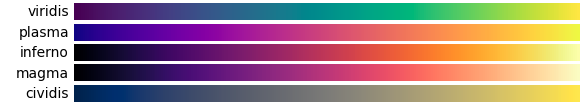
\includegraphics[width=.7\linewidth]{obrazky/sequential.png}
    \caption{Sequential colormap\cite{colormap}}
    \label{fig:colormap.seq}
\end{figure}

\begin{figure}[h!]
    \centering
    
\includegraphics[width=.7\linewidth]{obrazky/cyclic.png}
    \caption{Examples of cyclic colormaps\cite{colormap}}
    \label{fig:colormap.cyc}
\end{figure}


\begin{figure}[h!]
    \centering
    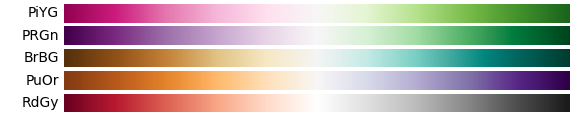
\includegraphics[width=.7\linewidth]{obrazky/diverging.png}
    \caption{Examples of diverging colormaps\cite{colormap}}
    \label{fig:colormap.div}
\end{figure}


\begin{figure}[h!]
    \centering
    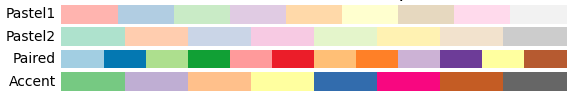
\includegraphics[width=.7\linewidth]{obrazky/qualitative.png}
    \caption{Examples of qualitative colormaps\cite{colormap}}
    \label{fig:colormap.qua}
\end{figure}



\section{Prototype}\label{txt.design.frontend.prototype}

To pitch ideas and show the design, a prototype was made. This prototype was not a final working application. The prototype was built with the Svelte framework for its high performance and fast development; see Section \ref{txt.design.frontend.svelte}. The prototype used Flowbite components\footnote{\url{https://flowbite-svelte.com/}} as they make it easy to create stylized web pages. The web page is divided into Svelte components. The main component is the waterfall graph on the left side of the screen and the control panel on the right side. Layout was done with svelte-layouts\footnote{\url{https://www.npmjs.com/package/svelte-layouts}} package. 

Uploading files into the browser using REST API was also tested. Python's \verb|http.server| was used as the back-end. When fetching files into a browser from local storage using HTTP, it is necessary to allow Cross-Origin Resource Sharing (CORS) because browsers restrict this feature for security reasons. Some resources like CSS, Web Fonts, and WebGL textures have enabled CORS. For sending HDF5 files to the browser, a special HTTP header has to be added on the server side. Without this feature, the browser would throw an error into the JavaScript console. CORS is not used for the later stages and implementation because we are not uploading whole HDF5 files.

\begin{figure}[h]
    \centering
    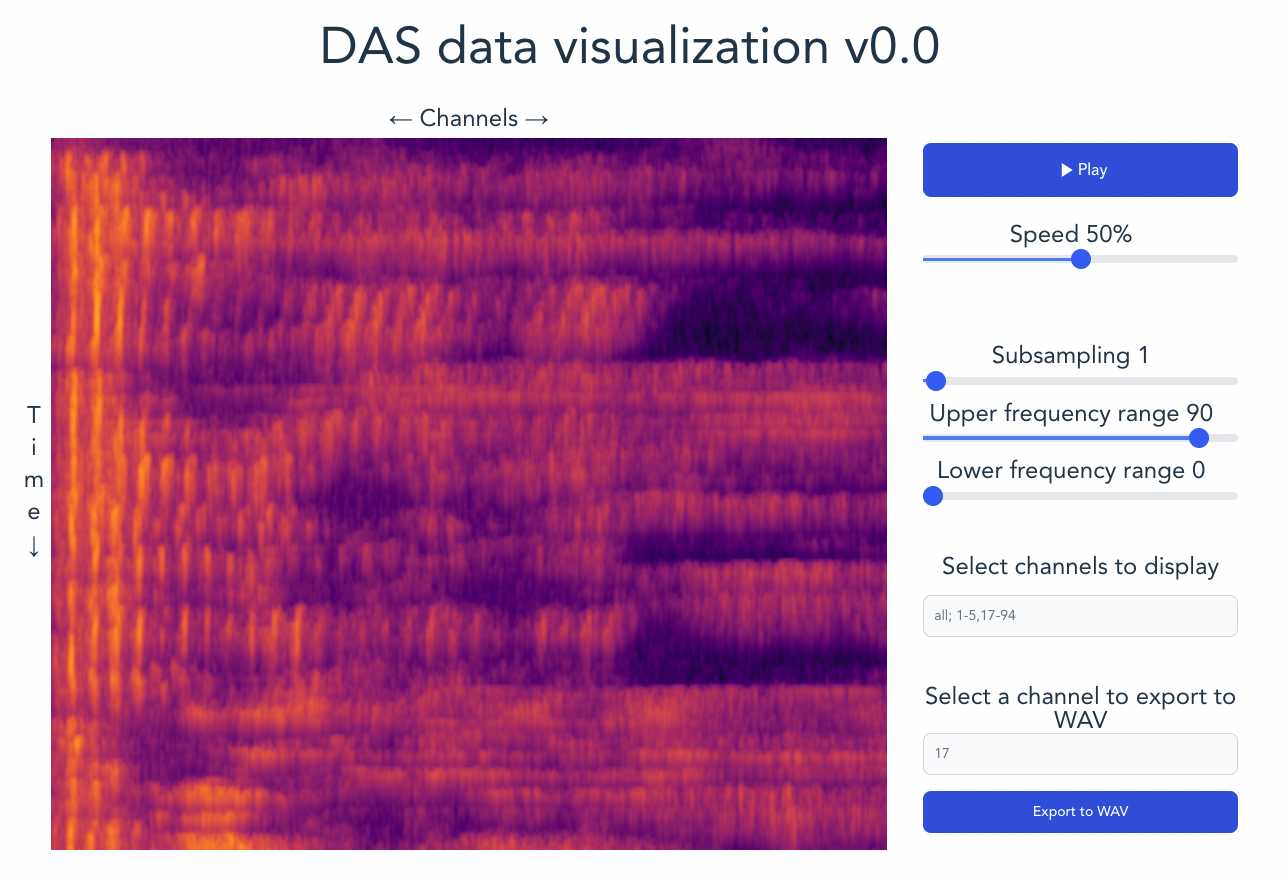
\includegraphics[width=\linewidth]{obrazky/svelte_prototype.png}
    \caption{Prototype of DAS visualization application}
    \label{fig:prototypesvelte}
\end{figure}

%%% Vložení souboru 'text/vysledky' s popisem vysledků práce
% (rozdělte na více souborů či kapitol, pokud je vhodné)
\chapter{Implementation of DAS visualization application}\label{txt.implementation}

This chapter provides an implementation overview of the DAS visualization application. Based on the previous chapters, we put everything together and created an application for data processing and visualization. The whole application consists of two main parts a Python back end and a JavaScript front end. 

\section{Python back-end application implementation}\label{txt.implementation.python}

The back-end is written in the programming language Python3.10\footnote{\url{https://www.python.org/}} was chosen. Python is a~great language for scientific use, data visualization, and graph plotting, which is the goal of this work. The most significant advantage comes from the availability of scientific libraries. 

To run the application, creating a virtual environment and installing all the dependencies in that environment is advisable. Installation steps can be found in Attachments \ref{atach:dependencies}. The application consists of multiple files, as seen in \ref{dir:filestructure.python}. 

\bigskip
Python back-end file structure:

{\small
%
\label{dir:filestructure.python}
\dirtree{%.
.1 optasense\_visualizer.
.2 app.py\DTcomment{Python script to run the application}.
.2 requirements.txt\DTcomment{Dependencies}
.2 src/\DTcomment{Folder with source files}.
.3 file\_reader.py\DTcomment{Opens and reads HDF5 files}.
.3 message\_classes.py\DTcomment{Data classes for incoming messages}.
.3 optasense\_server.py\DTcomment{Back-end part of application}.
.3 range\_parser.py\DTcomment{Functions for parsing channels}.
.3 spectral\_analysis.py\DTcomment{Functions for processing data}.
.3 streaming.py \DTcomment{Managing data streaming}.
}
}
\bigskip


The application is started by calling \verb|python3 app.py --port 8001|. Everything runs inside with the use of \textit{asyncio} library. The \textit{app.py} file parses arguments with the use of \textit{argparse} library. The only argument is the optional \textit{port} argument. The default value is 8001, which is later used by \textit{websocket}. Websocket uses \textit{async for} waiting for messages from the client side. Incoming messages are in JSON format. Every message has a \textit{type} which determines the incoming message. Messages are parsed using \textit{MessageParser} class, which implements a \textit{factory object}.
\textit{Factory} object is one of the most used object-oriented design patterns. It creates objects without revealing the logic to the client. The only implemented method is \verb|parse()|, which reads the type and then creates one of the message classes and returns it. Each message corresponds to its message class. For ease of programming, \textit{dataclasses} module was used. It provides functions and a decorator for the automatic generation of special methods (\verb|__init__()| or \verb|__repr__()|). There are 6 message dataclasses \textit{InitApp}, \textit{FindFiles}, \textit{OpenFile}, \textit{Streaming}, \textit{Properties} and \textit{ChannelSelection}, see Figure \ref{fig:uml}. When the message parsing fails, it raises an \verb|UnknownMessageException|. The exception is thrown away as we do not want to terminate execution whenever an incorrect message is received.

Message classes and the factory object \verb|MessageFactory| are in the \textit{message\_classes.py} file with an \textit{Exception} class \verb|UnknownMessageException|.

\begin{figure}
    \centering
    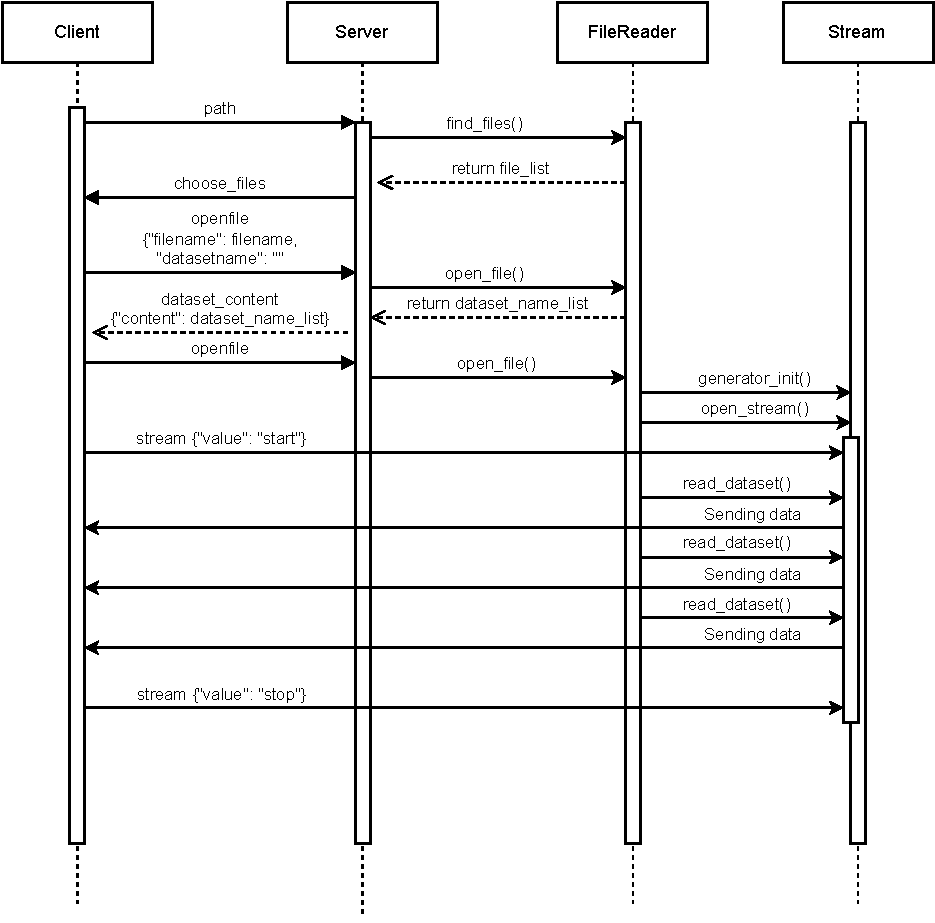
\includegraphics{pdf/websocketcomm.drawio.pdf}
    \caption{UML diagram of the back-end}
    \label{fig:uml}
\end{figure}

An example of an incoming message from the client received by the server:
\begin{verbatim}
{
    'type': 'path',
    'path': '/Users/user/Documents/',
    'suffix': '.h5'
}
\end{verbatim}

Next, the MessageFactory checks the message \verb|type| - \textit{"path"} corresponds to \textit{FindFiles} class and returns it. The message class is then saved as a server state. Each message class has its own \textit{if} statement with its behavior. Not to be confused, the behavior is defined outside of the class. It is not implemented in the data class itself.

\textit{FindFiles} is the first message sent from the client 

\subsection{Program implementation of HDF5 to WAV}\label{lab:hdftowav}\label{txt.implementation.wav}

This part of the project aims to create an application for reading data from the \ac{das} system and converting the data to the \verb|.wav| audio file format.

The opening of \verb |.h5| files is done with \verb|h5py| library\footnote{\url{https://www.h5py.org/}}. For working with dataset data types, \verb|numpy|\footnote{\url{https://numpy.org/}} library is used. The function for interpolating arrays to a~certain range is also used \verb|interp|. Lastly, to convert the signal data to \verb|.wav| audio format \verb|scipy| library is used specifically \verb|io| module function \verb|wavfile|. To read all options and input arguments, the \verb|argparse| library is used\footnote{\url{https://docs.python.org/3/library/argparse.html}}.

\begin{figure}
    \centering
    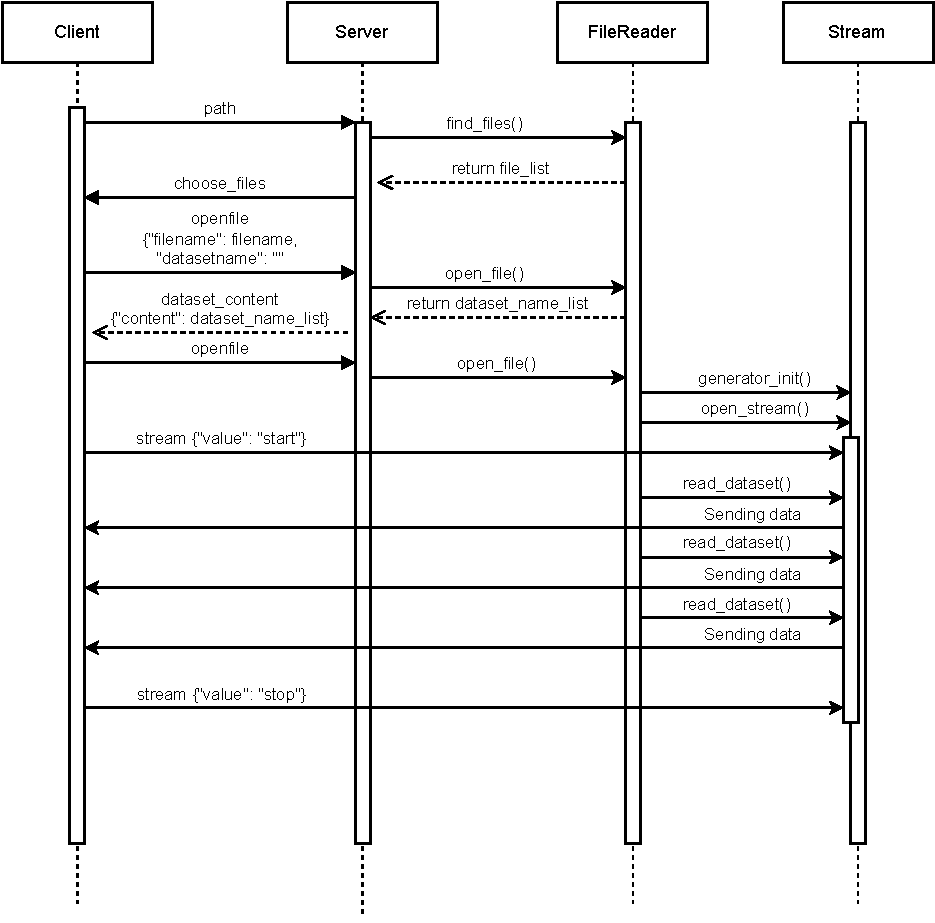
\includegraphics{pdf/websocketcomm.drawio.pdf}
    \caption{UML diagram of the back-end}
    \label{fig:uml}
\end{figure}

\subsection{Reading HDF5 file}\label{txt.implementation.reading}

The sample file recorded in the OptaSense ODH-F is in HDF5 file format. As \ac{hdf} files have a~user-defined structure on the application layer and in the binary form, it is hard to say what is actually in the file. To better understand the contents of the \verb|.h5| file, \verb|h5dump| was performed and a conversion to JSON\footnote{\url{https://www.json.org/json-en.html}} was also performed by the \verb|h5tojson| program\footnote{\url{https://hdf5-json.readthedocs.io/en/latest/tools/h5json.html}}. The JSON file is quite large - the original HDF5 file is only \qty{52,7}{MB}, and the JSON file is \qty{946,6}{MB}. The dump text file is half the size and provides the same information, but the datasets are harder to understand, but the whole file is only half the size of the JSON file at ``only'' \qty{420}{MB}. The JSON format is much easier to read. The structure of the file is divided into three parts:

\begin{itemize}
    \item \textit{apiVersion} - 1.1.1 version of API
    \item \textit{datasets} - Contain all the datasets organized by their UUID\footnote{Universally unique identifier} that are defined in the groups section. There is also an \textit{alias} that is in the format of a Unix-based system path, for example, \verb|"/Acquisition/Raw[0]/Custom/SampleCount"|. Other properties define the shape and type of stored data. In this case, the properties are shown in the table \ref{tab:file_details}.
    \item \textit{groups} - Groups are named by a UUID. The group object has:
        \begin{itemize}
            \item \textit{alias} - Unix-like name; the first is root ``/'' group
            \item \textit{attributes} - define the type, name, and shape of the value of the attribute, which is a string \verb|979bb2ac-99bf-4cb5-b410-5c16cd7872dc|
            \item \textit{links} - links to other groups that create a treelike structure. The link object contains the class of a link (e.g., H5L\_TYPE\_HARD for hard link), the \textit{collection} property telling that it is a group, and the name of the group. The group object also contains other important metadata, such as measurement settings. All important details are given in the table \ref{tab:file_details}
        \end{itemize}
\end{itemize}

There is a~library for reading \ac{hdf} files written in Python called \verb|h5py|. To read the \ac{hdf} file's contents, a~function was created called \verb|get_dataset_path()|, which recursively looks for all groups according to their name provided by the \verb|.keys()| method, in the dataset. The result of this function is propagated through recursion and saved in Python \verb|set()| built-in type. The user can then choose which one is the suitable dataset to use because there is probably more than one dataset. When calling the program, the user can save the string and use it as an argument. This saves time in searching for the contents of the file.

This is the data structure of the DAS file from the OptaSense Interrogator:

\bigskip
DAS output file structure in \ac{hdf} format
{\small
%
\label{dir:filestructure}
\dirtree{%.
.1 /\DTcomment{root}.
.2 Acquisition\DTcomment{Recorded data}.
.3 Custom\DTcomment{Empty}.
.3 Raw[0]\DTcomment{HDF5 group (3 members)}.
.4 Custom\DTcomment{HDF5 group (1 members)}.
.5 SampleCount\DTcomment{HDF5 dataset, shape (332032,), type "<i8">}.
.4 RawData[0]\DTcomment{HDF5 dataset, shape (100, 332032), type "<i2">}.
.4 RawDataTime\DTcomment{HDF5 dataset, shape (332032,), type "<i8">}.
}
}
\bigskip

The type of explanation in \ref{dir:filestructure} is \verb|i8|, which is \verb|numberpy.int64|. \verb|SampleCount| contains numbering of all samples, \verb|RawDataTime| contains time, and \verb|RawData[0]| contains sensor data we need to read in the following steps; see \ref{txt.design.datapprocessing}. More details are provided in Table \ref{tab:file_details}.

All important HDF5 attributes are shown in the table \ref{tab:file_details}. It contains metadata about the datasets, data dimensions, number of channels, kinds of filters used, time information, length of pulses, laser wavelength, and more. Some properties can be derived from those in the table. The capture duration can be calculated from the start and end of the capture, which is \qty{10,376}{\second}.

\subsection{Data processing for converting raw HDF5 data to WAV}\label{txt.implementation.processing}

The data have 100 channels with \textit{N} samples, in this example \qty{332032}{samples} saved in \verb|/Acquisition/Raw[0]/RawData[0]|, see the file structure in \ref{dir:filestructure}. The function \verb|scipy.io.wavfile.write()| saves samples to a file, and the data need more processing before the function can be called. After the data are read from the file, it is saved into \verb|samples| variable of type \verb|numpy.array| it is then processed in 4 steps as preparation for saving into \verb|.wav| file. The steps are:

\begin{enumerate}
    \item \textbf{Channel selection} - only channel one can be selected.
    \item \textbf{Data interpolation} - The original data have a terrible value range from -24838 to -30758, triggering an exception when writing the data into a \verb|.wav| file. The \verb|numpy.interp()|\footnote{\url{https://numpy.org/doc/stable/reference/generated/numpy.interp.html}} function interpolates the data into the range of the maximum and minimum values specified in this case by the \qty{16}{bit} PCM\footnote{Pulse Code Modulation}, which can be written to WAV file by \verb|wavfile| module.
    \item \textbf{Resampling} - as the data are recorded at a certain sampling frequency, in this case, \qty{10}{\kHz}, resampling by the function \verb|scipy.signal.resample() |\footnote{\url{https://docs.scipy.org/doc/scipy/reference/generated/scipy.signal.resample.html}} is necessary. The right number of samples is calculated by the formula \ref{formula:sampling}.
    \item \textbf{Retyping} - the resampled data need to be in the correct format, and since the interpolation was done in the range of \verb|int16|, the output type of choice is the same \verb|samples.astype(np.int16)|.
\end{enumerate}

\begin{equation}
    \label{formula:sampling}
    numSamples = \frac{44100}{fs.len(samples)}
\end{equation}


\begin{table}[]
    \centering
    \begin{tabular}{|c|c|c|c|}
    \hline
    \textbf{Data type} & \textbf{Minimum value} & \textbf{Maximum value} & \textbf{WAV format} \\
    \hline
    float32 & -1.0 & +1.0 & 32-bit floating-point \\ \hline
    int32 & -2147483648 & +2147483647 & 32-bit PCM \\ \hline
    int16 & -32768 & +32767 & 16-bit PCM \\ \hline
    uint8 & 0 & 255 & 8-bit PCM \\
    \hline
    \end{tabular}
    \caption{WAV compatible types}
    \label{tab:my_label}
\end{table}





\section{Frontend client application}\label{txt.implementation.svelte}
\subsection{Svelte components}\label{txt.implementation.components}
\subsection{Svelte stores}\label{txt.implementation.stores}



%%% Vložení souboru 'text/zaver' se závěrem
\chapter*{Conclusion}
\phantomsection
\addcontentsline{toc}{chapter}{Conclusion}

The main goal of this work was to study the~DAS system and its output files in~the~HDF5 file format. As for the~implementation part, the~goal was to create a~multi-platform application capable of displaying the~data from the~DAS interrogator, processing it, and displaying it in a~suitable form. The visualization should be able to play and pause the~animation of the~flowing data, also with the~ability to convert the~data into an audio file.  

In the~theoretical part, the~principles of optical reflectometry were explained, as well as different types of light scattering - Mie scattering, Rayleigh scattering, Raman scattering, and Brillouin scattering. the~inner workings of the~DAS system and methods like \ac{generalotdr} and \ac{otdr} were also studied. The output file format HDF5 was carefully examined with objects such as Datasets, Groups, Attributes, and Links. The output file structure of the~DAS system OptaSense ODH-F was shown in a~readable form. The existing technology was studied with available software for the~front-end and server side. Real-time capabilities were also discussed with the~data bandwidth requirements. A~prototype was created and written in~Svelte to showcase the~application's design with a~waterfall graph and HTML elements to set properties for display. 

In the~design section, we discuss software requirements and the~basic back-end technologies used later in the~implementation section, such as WebSockets and reading HDF5 files. The front-end technologies for data visualization based on Canvas and SVG graphics were discussed. The basics of the~Svelte framework were introduced.

A web application was created with a~server written in Python and a~client using the~Svelte framework. The back end can read and process the~data in HDF5 file format. The back-end communicates with the~client side using WebSockets. A~simple message system was created for this purpose. The client allows the~user to choose the~file and the~dataset, as well as properties like speed choosing a~colormap and channels to display. The visualization can be started, stopped, and replayed. There is also a~feature to download the~image currently on display.

% In the~last section the~software design of a~real-time application for the~DAS system was discussed. 


% The work can be used as a~resource for creating an application for data visualization in the~browser. The next step is to create fully functional web application - with its server-side written in Python sending data using WebSockets to the~front-end client application written in Svelte.

The application in this state is a~one-page website; the~next step would be to incorporate it into the~SvelteKit framework, allowing page routing. This should be pretty straightforward. Future work can include further improving the~visualization, including zooming and data selection features, either by creating custom \texttt{<canvas>} rendering, SVG rendering with D3js, or using existing libraries such as Plotly. It~might be useful to have multiple algorithms to choose from when processing the~raw DAS data. Although we tried a~few methods for data processing, we have chosen one, and there is no selection possible at this stage.





% \section{}

% The semestral part of the~thesis studies DAS principles

% and the output format of the deployed system, 

% \section{Implementation}

% followed by an implementation of conversion from data to audio signal (in WAV format). 

% \subsection{Real-time possibilities}

% This part also investigates the possibilities of real-time data analysis



% Práce je zaměřena na analýzu dat z optického distribuovaného akustického senzorického (DAS) systému ve formátu HDF5. V semestrální práci student prostuduje princip DAS systém a~jeho výstupy (HDF5 archivy) s detailním popisem formátu HDF5. Následně navrhne program pro převod dat do akustické podoby (WAV) a~popíše možnosti realizace programu v reálném čase. V diplomové práci bude navrženo grafické rozhraní zobrazující data v čase s možnostmi úprav os grafu. Výsledek bude otestován s reálným DAS systémem a~fakultním optickým senzorickým polygonem.




% Info o systeme co pouzivaju v tyme
% 	HW info
% 	outputformat - popisat atributy, kanaly, a~celkovo ako to uklada to toho hdf5ky




% Obsah:
% ako to funguje
% existujuci HW


%%% Vložení souboru 'text/literatura' se seznamem zdrojů
% Pro sazbu seznamu literatury použijte jednu z následujících možností

%%%%%%%%%%%%%%%%%%%%%%%%%%%%%%%%%%%%%%%%%%%%%%%%%%%%%%%%%%%%%%%%%%%%%%%%%
%1) Seznam citací definovaný přímo pomocí prostředí literatura / thebibliography

\begin{thebibliography}{99}

\bibitem{WangYu2017RDVM}

WANG, Yu, Baoquan JIN, Yuncai WANG, Dong WANG, Xin LIU, Qing BAI: \emph{Real-Time Distributed Vibration Monitoring System Using $\Phi$-OTDR}. IEEE sensors journal [online]. PISCATAWAY: IEEE, 2017, 17(5), 1333-1341 [cit. 2022-11-22]. ISSN 1530-437X. Accessible at: doi:10.1109/JSEN.2016.2642221

\bibitem{dasKislov}
KISLOV, K. V. a V. V. GRAVIROV: \emph{Distributed Acoustic Sensing: A New Tool or a New Paradigm. Seismic instruments} [online]. Moscow: Pleiades Publishing, 2022, 58(5), 485-508 [cit. 2022-11-22]. ISSN 0747-9239. Accessible at: doi:10.3103/S0747923922050085

\bibitem{dasseismic}
PARKER, Tom, SHATALIN, Sergey, FARHADIROUSAN Mahmoud: \emph{Distributed Acoustic Sensing – a new tool for seismic applications}. Earthdoc [online]. [cit. 2022-11-22]. Accessible at \(<\)\url{https://doi.org/10.3997/1365-2397.2013034}\(>\)

\bibitem{gabai}
GABAI, Haniel, and AVISHAY Eyal: \emph{On the sensitivity of distributed acoustic sensing.} Optics letters vol. 41,24 (2016): 5648-5651. [online]. [cit. 2022-11-22] doi:10.1364/OL.41.005648

\bibitem{wangprogress}
WANG Z, LU B, YE Q, CAI H.: \emph{Recent Progress in Distributed Fiber Acoustic Sensing with $\Phi$-OTDR}. Sensors (Basel). 2020 Nov 18;20(22):6594. doi: 10.3390/s20226594. PMID: 33218051; PMCID: PMC7698859.

\bibitem{kislov_das_newparadigm}
KISLOV, K. V. a V. V. GRAVIROV.: \emph{Distributed Acoustic Sensing: A New Tool or a New Paradigm. Seismic instruments} [online]. Moscow: Pleiades Publishing, 2022, 58(5), 485-508 [cit. 2022-11-25]. ISSN 0747-9239. Accessible at: doi:10.3103/S0747923922050085

\bibitem{hdf5doc}
\emph{The HDF5 Data Model and File Structure} HDF Group [cit. 2022-12-08]. Accessible at \(<\)\url{https://docs.hdfgroup.org/hdf5/develop/_h5_d_m__u_g.html}\(>\).

\bibitem{hdfrest}
HEBER G.: \emph{RESTful HDF5} The HDF Group [cit. 2022-12-08].
\(<\)\url{https://support.hdfgroup.org/pubs/papers/RESTful_HDF5.pdf}\(>\).

\bibitem{seismic}
HORNMAN, J.C.: \emph{Field trial of seismic recording using distributed acoustic sensing with broadside sensitive fibre-optic cables.} Geophysical Prospecting [online]. 2017, 65(1), 35-46 [cit. 2022-12-06]. ISSN 0016-8025. Accessible at: doi:10.1111/1365-2478.12358

\bibitem{progress}
BAO, Xiaoyi a Liang CHEN.: \emph{Recent Progress in Distributed Fiber Optic Sensors}. Sensors (Basel, Switzerland) [online]. BASEL: Mdpi, 2012, 12(7), 8601-8639 [cit. 2022-12-08]. ISSN 1424-8220. Accessible at: doi:10.3390/s120708601

\bibitem{dasrayleigh}
PALMIERI, Luca; SCHENATO, Luca. Distributed optical fiber sensing based on Rayleigh scattering. The Open Optics Journal, 2013, 7.1.

\bibitem{ytossix}
OptaSense OS6 Visualization Software Demo. YouTube, uploaded by OptaSense, 22 June 2021, \(<\)\url{https://www.youtube.com/watch?v=6-hj1ySERIA}\(>\).

\bibitem{websock}
Melnikov, A., Fette, I.: \emph{The WebSocket Protocol}. RFC Editor. [online] [cit. 2022-08-12]. Accessible at: \(<\)\url{https://doi.org/10.17487/RFC6455}\(>\).

\bibitem{cors} 
\emph{Cross-Origin Resource Sharing (CORS)} mozilla.org [cit. 2022-12-08]. Accessible at \(<\)\url{https://developer.mozilla.org/en-US/docs/Web/HTTP/CORS}\(>\).


% @misc{rfc6455,
%     series =    {Request for Comments},
%     number =    6455,
%     howpublished =  {RFC 6455},
%     publisher = {RFC Editor},
%     doi =       {10.17487/RFC6455},
%     url =       {https://www.rfc-editor.org/info/rfc6455},
%         author =    {Alexey Melnikov and Ian Fette},
%     title =     {{The WebSocket Protocol}},
%     pagetotal = 71,
%     year =      2011,
%     month =     dec,
%     abstract =  {The WebSocket Protocol enables two-way communication between a client running untrusted code in a controlled environment to a remote host that has opted-in to communications from that code. The security model used for this is the origin-based security model commonly used by web browsers. The protocol consists of an opening handshake followed by basic message framing, layered over TCP. The goal of this technology is to provide a mechanism for browser-based applications that need two-way communication with servers that does not rely on opening multiple HTTP connections (e.g., using XMLHttpRequest or \textless{}iframe\textgreater{}s and long polling). {[}STANDARDS-TRACK{]}},
% }





% \bibitem{sr02/2009}
% 		VUT v~Brně:
%     \emph{Úprava, odevzdávání a zveřejňování vysokoškolských kva\-li\-fi\-kač\-ních prací na VUT v~Brně}\/ [online].
% 		Směrnice rektora č.\,2/2009.
% 		Brno: 2009, po\-sled\-ní aktualizace 24.\,3.\,2009 [cit.\,23.\,10.\,2015].
%     Dostupné z~URL:\\
%     <\url{https://www.vutbr.cz/uredni-deska/vnitrni-predpisy-a-dokumenty/smernice-rektora-f34920/}>.

% \bibitem{CSN_ISO_690-2011}
%     \emph{ČSN ISO 690 (01 0197) Informace a dokumentace -- Pravidla pro bibliografické odkazy a citace informačních zdrojů.}
%     40 stran. Praha: Český normalizační institut, 2011.

% \bibitem{CSN_ISO_7144-1997}
%     \emph{ČSN ISO 7144 (010161) Dokumentace -- Formální úprava disertací a podobných dokumentů.}
%     24 stran. Praha: Český normalizační institut, 1997.

% \bibitem{CSN_ISO_31-11}
%     \emph{ČSN ISO 31-11 Veličiny a jednotky -- část 11: Matematické znaky a značky používané ve fyzikálních vědách a v~technice.}
%     Praha: Český normalizační institut, 1999.

% \bibitem{BiernatovaSkupa2011:CSNISO690komentar}
%     BIERNÁTOVÁ, O., SKŮPA, J.:
%     \emph{Bibliografické odkazy a citace dokumentů dle ČSN ISO 690 (01 0197) platné od 1.\,dubna 2011}\/ [online].
%     2011, poslední aktualizace 2.\,9.\,2011 [cit. 19.\,10.\,2011].
%     Dostupné z~URL:
%     \(<\)\url{http://www.citace.com/CSN-ISO-690.pdf}\(>\)
%    \(<\)\href{http://www.boldis.cz/citace/citace.html}{http://www.boldis.cz/citace/citace.html}\(>\).

% \bibitem{pravidla}
%     \emph{Pravidla českého pravopisu}.
%     Zpracoval kolektiv autorů. 1.\ vydání.
%     Olomouc: FIN PUB\-LISH\-ING, 1998. 575 s. ISBN 80-86002-40-3.

% \bibitem{Walter1999}
% 	WALTER, G.\,G.; SHEN, X.
% 	\emph{Wavelets and Other Orthogonal Systems}.
% 	2. vyd. Boca Raton: Chapman\,\&\,Hall/CRC, 2000. 392~s. ISBN 1-58488-227-1

% \bibitem{Svacina1999IEEE}
% 	SVAČINA, J.
% 	Dispersion Characteristics of Multilayered Slotlines -- a Simple Approach.
% 	\emph{IEEE Transactions on Microwave Theory and Techniques},
% 	1999, vol.\,47, no.\,9, s.\,1826--1829. ISSN 0018-9480.

% \bibitem{RajmicSysel2002}
%     RAJMIC, P.; SYSEL, P.
%     Wavelet Spectrum Thresholding Rules.
%     In \emph{Proceedings of the International Conference Research in Telecommunication Technology},
%     Žilina: Žilina University, 2002. s.\,60--63. ISBN 80-7100-991-1.

\end{thebibliography}


%%%%%%%%%%%%%%%%%%%%%%%%%%%%%%%%%%%%%%%%%%%%%%%%%%%%%%%%%%%%%%%%%%%%%%%%%
%%2) Seznam citací pomocí BibTeXu
%% Při použití je nutné v TeXnicCenter ve výstupním profilu aktivovat spouštění BibTeXu po překladu.
%% Definice stylu seznamu
%\bibliographystyle{unsrturl}
%% Pro českou sazbu lze použít styl czechiso.bst ze stránek
%% http://www.fit.vutbr.cz/~martinek/latex/czechiso.tar.gz
%%\bibliographystyle{czechiso}
%% Vložení souboru se seznamem citací
%\bibliography{text/literatura}
%
%% Následující příkaz je pouze pro ukázku sazby literatury při použití BibTeXu.
%% Způsobí citaci všech zdrojů v souboru literatura.bib, i když nejsou citovány v textu.
%\nocite{*}

%%% Vložení souboru 'text/zkratky' se seznam použitých symbolů, veličin a zkratek
\cleardoublepage
\chapter*{\listofabbrevname}
\phantomsection
\addcontentsline{toc}{chapter}{\listofabbrevname}

\begin{acronym}[KolikMista]
        \acro{adm}
            [ADM]
            {Abstract Data Model}
        \acro{otdr}
            [$\Phi$-OTDR]
            {Phase-Sensitive Optical Time Domain Reflectometry}
        \acro{das}
            [DAS]
            {Distributed Acoustic Sensing}

        \acro{dss}
            [DSS]
            {Distributed Strain Sensing}

        \acro{dts}
            [DTS]
            {Distributed Temperature Sensing}
        \acro{dvs}
            [DVS]
            {Distributed Vibration Sensing}
        % \acro{}
        %     []
        %     {Distributed  Sensing}
        % \acro{}
        %     []
        %     {Distributed  Sensing}
   
        \acro{generalotdr}
            [OTDR]
            {Optic Time Domain Reflectometry}
        \acro{fft}
            [FFT]
            {Fast Fourier Transformation}
	   \acro{hdf}
            [HDF5]
            {Hierarchical Data Format v5}
        \acro{ofdr}
            [OFDR]
            {Optic Frequency Domain Reflectometry}
        \acro{sps}
            [SPS]
            {samples per second}

        \acro{svg}
            [SVG]
            {Scalable Vector Graphics}
        \acro{dthree}[D3.js]{Data-Driven Documents}
        \acro{dom}{DOM}{Document Object Model}
											% rozvinutí zkratky
	% \acro{zkTemp}		% název
	% 	[Šířka levého sloupce Seznamu symbolů a zkratek]								% zkratka
	% 	{je určena šířkou parametru prostředí \texttt{acronym} (viz řádek~1 výpisu zdrojáku na~str.\,\pageref{lst:zkratky})}
	% 										% rozvinutí zkratky

	% \acro{zkDummy}
	% 	[KolikMista]
	% 	{pouze ukázka vyhrazeného místa}

	% \acro{DSP}		% název/zkratka
	% 	{číslicové zpracování signálů -- Digital Signal Processing}
	% 										% rozvinutí zkratky
	% %%% bsymfvz
	% \acro{symfvz}						% název
	% 	[\ensuremath{f_\textind{vz}}] % symbol
	% 	{vzorkovací kmitočet}					% popis
	% %%% esymfvz

\end{acronym}


%%% Začátek příloh
\appendix

%%% Vysázení seznamu příloh
% (vynechejte, pokud máte dvě nebo méně příloh)
\listofappendices

%%% Vložení souboru 'text/prilohy' s přílohami
% Obvykle je přítomen alespoň popis co najdeme na přiloženém médiu
\chapter{Installing dependencies}\label{atach:dependencies}

Using a virtual environment is suggested and installing all dependencies in the environment.

\begin{verbatim}
    python3 -m venv env
    source env/bin/activate
    pip3 install -r requirements
\end{verbatim}

\section{Optasense visualizer application usage}\label{usage}

To run the application it is necessary to have an environment set up and all dependencies installed.
\textit{} \newline
Run the server part of the application:
\begin{verbatim}
    python3 app.py
\end{verbatim}

\textit{} \newline
The application usage:

\begin{verbatim}
usage: app.py [-h] [--port PORT]

DAS file visualization software. Server application.

options:
  -h, --help   show this help message and exit
  --port PORT  Port number for websocket.
\end{verbatim}


\section{Svelte}\label{attach:svelte}
\textit{} \newline
To create a Svelte application from template:

\begin{verbatim}
    npm create svelte@latest myapp
\end{verbatim}

Run the client on the localhost:

\begin{verbatim}
    npm run dev
\end{verbatim}

To run a build call:

\begin{verbatim}
    npm run build
\end{verbatim}

The output will be saved in \textit{/dist} folder. To run the application from there, run Python script in the project's client folder:

\begin{verbatim}
    python3 server.py
\end{verbatim}

Server created this way is a simple Flask server.

\chapter{OptaSense DAS system measurement\newline properties}\label{attach:properties}

\begin{table}[h]
    \centering
    \begin{tabular}{|c|c|}
    \hline
        \textbf{Property} & \textbf{Value} \\ \hline
    \multicolumn{2}{|c|}{\textbf{/Acquisition}} \\ \hline
        MaximumFrequency & 16000 \\ \hline
        MinimumFrequency & 0 \\ \hline
        NumberOfLoci & 100 \\ \hline
        PulseRate & \qty{32}{} \\ \hline
        PulseWidth & \qty{20}{\ns} \\ \hline
        SpatialSamplingInterval & \qty{1.02095}{\meter} \\ \hline
        StartLocusIndex & 600 \\ \hline
    \multicolumn{2}{|c|}{\textbf{/Acquisition/Custom}} \\ \hline
        Data Width (Bits) & 16 bits \\ \hline
        FPGA infromation & Type and settings \\ \hline
        FPGA Drawing Number & 4802701 \\ \hline
        FPGA Version & 1.2 \\ \hline
        Fibre Refractive Index & 1.468199968338 \\ \hline
        GPS Enabled & True \\ \hline
        Laser Wavelength (nm) & 1550 \\ \hline
        Num Output Channels & 100 \\ \hline
        Ping Period (CSU) & 3125 \\ \hline
        Pulse Width (CSU) & 2 \\ \hline
        Sequencer Clock (MHz) & 100 MHz \\ \hline
        Sequencer Mode & 1 \\ \hline
    \multicolumn{2}{|c|}{\textbf{/Acquisition/Raw[0]}} \\ \hline
        OutputDataRate & 32000  \\ \hline
        NumberOfLoci & 100  \\ \hline
        RawDescription & Single Pulse, SR: 1.5, OCP: 1  \\ \hline
        StartLocusIndex & 600  \\ \hline

    \end{tabular}
    \caption{HDF5 groups and their attributes from the data file.}
    \label{tab:file_details}
\end{table}
\begin{table}[]
    \centering
    \begin{tabular}{|c|c|}
    \hline
    \textbf{Property} & \textbf{Value} \\ \hline
        
    \multicolumn{2}{|c|}{\textbf{/Acquisition/Raw[0]/Custom/SampleCount}} \\ \hline
        Filters & shuffle and deflate \\ \hline
        maximum dimensions & 6451612 \\ \hline
        shape (number of samples) & 332032 \\ \hline
        type & \makecell{64-bit integer} \\ \hline
        
    \multicolumn{2}{|c|}{\textbf{/Acquisition/Raw[0]/RawData}} \\ \hline
        \makecell{Count \\ number of all values} & 33203200 \\ \hline
        Start time & 2021-08-31T16:22:39.739250Z \\ \hline
        End time & 2021-08-31T16:22:50.115218Z \\ \hline
        Filters & shuffle and deflate \\ \hline
        type & \makecell{64-bit integer} \\ \hline
        Shape & \makecell{100 channels \\ 332032 samples } \\ \hline
    \multicolumn{2}{|c|}{\textbf{/Acquisition/Raw[0]/RawDataTime}} \\ \hline
        Start time & 2021-08-31T16:22:39.739250Z \\ \hline
        End time & 2021-08-31T16:22:50.115218Z \\ \hline
        Filters & shuffle and deflate \\ \hline
        start index & 0 \\ \hline
        shape & 332032 \\ \hline
        type & \makecell{64-bit integer} \\
    \hline
    \end{tabular}
    \caption{HDF5 groups and their attributes from the data file.}
    \label{tab:file_details1}
\end{table}



\begin{table}[]
    \centering
    \begin{tabular}{|c|c|}
    \hline
    \textbf{Property} & \textbf{Value} \\ \hline
        
    \multicolumn{2}{|c|}{\textbf{/Acquisition}} \\ \hline
		MaximumFrequency & 10000.0 \\ \hline
		MinimumFrequency & 0.0 \\ \hline
		NumberOfLoci & 1700 \\ \hline
		PulseRate & 20000.0 \\ \hline
		PulseWidth & 20.0 \\ \hline
		PulseWidthUnit & ns \\ \hline
		SpatialSamplingInterval & 1.0209523 \\ \hline
		SpatialSamplingIntervalUnit & m \\ \hline
		StartLocusIndex & 0 \\ \hline
		TriggeredMeasurement & false \\ \hline
		VendorCode & \makecell{OptaSense IU Setup 1.8.6 \\ c9c23ad2ab20eb82641984e0e1205500228e9fba} \\ \hline
		schemaVersion & 2.0 \\ \hline
		uuid & bb17e24c-0c96-44d0-b4b0-a25a72db10e2 \\ \hline
        Filters & shuffle and deflate \\ \hline
        maximum dimensions & 6451612 \\ \hline
        shape (number of samples) & 332032 \\ \hline
        type & \makecell{64-bit integer} \\ \hline
    \multicolumn{2}{|c|}{\textbf{/Acquisition/Raw[0]}} \\ \hline
        \makecell{Count \\ number of all values} & 33203200 \\ \hline
		% Custom & <HDF5 group "/Acquisition/Raw[0]/Custom" (4 members)> \\ \hline
		% RawData & <HDF5 dataset "RawData": shape (1140000, 1700), type "<i2"> \\ \hline
		% RawDataTime & <HDF5 dataset "RawDataTime": shape (1140000,), type "<i8"> \\ \hline
		NumberOfLoci & 1700 \\ \hline
		OutputDataRate & 20000.0 \\ \hline
		RawDescription & b'Single Pulse, SR: 1.5, OCP: 1' \\ \hline
		StartLocusIndex & 0 \\ \hline
		uuid & b'34baa19e-cdde-48d7-8430-fbc9eb2187e6' \\ \hline
    \multicolumn{2}{|c|}{\textbf{/Acquisition/Raw[0]/RawData}} \\ \hline
		Count & 1938000000  \\ \hline
		Dimensions & array([time, locus], dtype='|S6')  \\ \hline
		PartEndTime & 2023-04-17T11:25:10.456750Z  \\ \hline
		PartStartTime & 2023-04-17T11:24:13.456800Z  \\ \hline
		StartIndex & 0  \\ \hline
    \hline
    \end{tabular}
    \caption{HDF5 groups and their attributes from the running data file.}
    \label{tab:filerunning}
\end{table}

\chapter{Printing the HDF5 data structure and metadata}

\begin{verbatim}
    h5dump -n running_2023-04-17T122413+0100.h5

    HDF5 "running_2023-04-17T122413+0100.h5" {
        FILE_CONTENTS {
         group      /
         group      /Acquisition
         group      /Acquisition/Custom
         group      /Acquisition/Raw[0]
         group      /Acquisition/Raw[0]/Custom
         dataset    /Acquisition/Raw[0]/Custom/GpBits
         dataset    /Acquisition/Raw[0]/Custom/GpsStatus
         dataset    /Acquisition/Raw[0]/Custom/PpsOffset
         dataset    /Acquisition/Raw[0]/Custom/SampleCount
         dataset    /Acquisition/Raw[0]/RawData
         dataset    /Acquisition/Raw[0]/RawDataTime
      }
    }


    
\end{verbatim}






% \section{Příkazy pro sazbu veličin a jednotek}

% \begin{table}[!h]
%   \caption[Přehled příkazů]{Přehled příkazů pro matematické prostředí }
%   \begin{center}
%   	\small
% 	  \begin{tabular}{|c|c|c|c|}
% 	    \hline
% 	    Příkaz    						& Příklad 					& Zdroj příkladu  							& Význam  \\
% 	    \hline\hline
% 	    \verb|\textind{...}|	& $\beta_\textind{max}$ 	& \verb|$\beta_\textind{max}$|	& textový index \\
% 	    \hline
% 	    \verb|\const{...}| 		& $\const{U}_\textind{in}$ 				& \verb|$\const{U}_\textind{in}$|		& konstantní veličina \\
% 	    \hline
% 	    \verb|\var{...}| 		& $\var{u}_\textind{in}$ & \verb|$\var{u}_\textind{in}$| & proměnná veličina \\
% 	    \hline
% 	    \verb|\complex{...}| 	& $\complex{u}_\textind{in}$ & \verb|$\complex{u}_\textind{in}$| & komplexní veličina \\
% 	    \hline
% 	    \verb|\vect{...}| 		& $\vect{y}$ 						& \verb|$\vect{y}$| & vektor \\
% 	    \hline
% 	    \verb|\mat{...}| 	& $\mat{Z}$ 						& \verb|$\mat{Z}$| & matice \\
% 	    \hline
% 	    \verb|\unit{...}| 		& $\unit{kV}$ 						& \verb|$\unit{kV}$|\quad či\ \, \verb|\unit{kV}| & jednotka \\
% 	    \hline
% 	  \end{tabular}
%   \end{center}
% \end{table}



% %\newpage
% \section{Příkazy pro sazbu symbolů}

% \begin{itemize}
%   \item
%     \verb|\E|, \verb|\eul| -- sazba Eulerova čísla: $\eul$,
%   \item
%     \verb|\J|, \verb|\jmag|, \verb|\I|, \verb|\imag| -- sazba imaginární jednotky: $\jmag$, $\imag$,
%   \item
%     \verb|\dif| -- sazba diferenciálu: $\dif$,
%   \item
%     \verb|\sinc| -- sazba funkce: $\sinc$,
%   \item
%     \verb|\mikro| -- sazba symbolu mikro stojatým písmem%
% 			\footnote{znak pochází z~balíčku \texttt{textcomp}}: $\mikro$,
% 	\item
% 		\verb|\uppi| -- sazba symbolu $\uppi$
% 			(stojaté řecké pí, na rozdíl od \verb|\pi|, což sází $\pi$).
% \end{itemize}
% %
% Všechny symboly jsou určeny pro matematický mód, vyjma \verb|\mikro|, jenž je\\ použitelný rovněž v~textovém módu.
% %$\upmikro$


% \chapter{Druhá příloha}

% \begin{figure}[!h]
%   \begin{center}
%     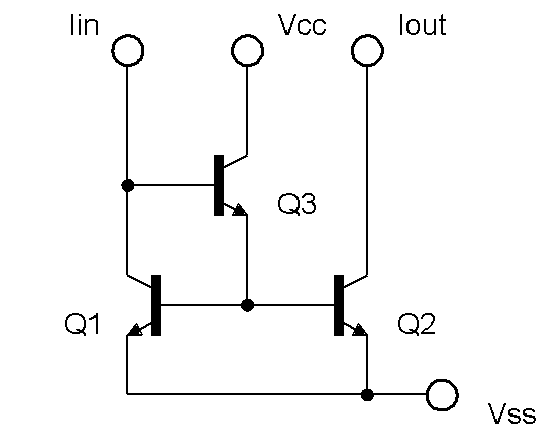
\includegraphics[scale=0.5]{obrazky/ZlepseneWilsonovoZrcadloNPN}
%   \end{center}
%   \caption[Alenčino zrcadlo]{Zlepšené Wilsonovo proudové zrcadlo.}
% \end{figure}

% Pro sazbu vektorových obrázků přímo v~\LaTeX{}u je možné doporučit balíček \href{https://www.ctan.org/pkg/pgf}{\texttt{TikZ}}.
% Příklady sazby je možné najít na \href{http://www.texample.net/tikz/examples/}{\TeX{}ample}.
% Pro vyzkoušení je možné použít programy QTikz nebo TikzEdt.




% \chapter{Příklad sazby zdrojových kódů}

% \section{Balíček \texttt{listings}}

% Pro vysázení zdrojových souborů je možné použít balíček \href{https://www.ctan.org/pkg/listings}{\texttt{listings}}.
% Balíček zavádí nové prostředí \texttt{lstlisting} pro sazbu zdrojových kódů, jako například:
% %
% \begin{lstlisting}[language={[LaTeX]TeX}]
% \section{Balíček lstlistings}
% Pro vysázení zdrojových souborů je možné použít
% 	balíček \href{https://www.ctan.org/pkg/listings}%
% 	{\texttt{listings}}.
% Balíček zavádí nové prostředí \texttt{lstlisting} pro
% 	sazbu zdrojových kódů.
% \end{lstlisting}
% %
% Podporuje množství programovacích jazyků.
% Kód k~vysázení může být načítán přímo ze zdrojových souborů.
% Umožňuje vkládat čísla řádků nebo vypisovat jen vybrané úseky kódu.
% Např.:

% \noindent
% Zkratky jsou sázeny v~prostředí \texttt{acronym}:
% \label{lst:zkratky}
% \lstinputlisting[language={[LaTeX]TeX},nolol,numbers=left, firstnumber=6, firstline=6,lastline=6]{text/zkratky.tex}
% %
% Šířka textu volitelného parametru \verb|KolikMista| udává šířku prvního sloupce se zkratkami.
% Proto by měla být zadávána nejdelší zkratka nebo symbol.
% Příklad definice zkratky \acs{symfvz} je na výpisu \ref{lst:symfvz}.

% \shorthandoff{-}
% \lstinputlisting[language={[LaTeX]TeX},frame=single,caption={Ukázka sazby zkratek},label=lst:symfvz,numbers=left,linerange={bsymfvz-\%\%\%\ esymfvz},includerangemarker=false]{text/zkratky.tex}
% \shorthandon{-}

% \noindent
% Ukončení seznamu je provedeno ukončením prostředí:
% \lstinputlisting[language={[LaTeX]TeX},nolol,numbers=left,firstnumber=26,linerange=26]{text/zkratky.tex}

% \vspace{\fill}

% \noindent
% {\bf Poznámka k~výpisům s~použitím volby jazyka \verb|czech| nebo \verb|slovak|:}\newline
% Pokud Váš zdrojový kód obsahuje znak spojovníku \verb|-|, pak překlad může skončit chybou.
% Ta je způsobená tím, že znak \verb|-| je v~českém nebo slovenském nastavení balíčku \verb|babel| tzv.\ aktivním znakem.
% Přepněte znak \verb|-| na neaktivní příkazem \verb|\shorthandoff{-}| těsně před výpisem a hned za ním jej vraťte na aktivní příkazem \verb|\shorthandon{-}|.
% Podobně jako to je ukázáno ve zdrojovém kódu šablony.


% \clearpage

% %\section{Výpis kódu prostředí Matlab}
% Na výpisu \ref{lst:priklad.vypis.kodu.Matlab} naleznete příklad kódu pro Matlab, na výpisu \ref{lst:priklad.vypis.kodu.C} zase pro jazyk~C.

% \lstnewenvironment{matlab}[1][]{%
% \iflanguage{czech}{\shorthandoff{-}}{}%
% \iflanguage{slovak}{\shorthandoff{-}}{}%
% \lstset{language=Matlab,numbers=left,#1}%
% }{%
% \iflanguage{slovak}{\shorthandon{-}}{}%
% \iflanguage{czech}{\shorthandon{-}}{}%
% }

% \begin{matlab}[frame=single,float=htbp,caption={Příklad Schur-Cohnova testu stability v~prostředí Matlab.},label=lst:priklad.vypis.kodu.Matlab,numberstyle=\scriptsize, numbersep=7pt]
% %% Priklad testovani stability filtru

% % koeficienty polynomu ve jmenovateli
% a = [ 5, 11.2, 5.44, -0.384, -2.3552, -1.2288];
% disp( 'Polynom:'); disp(poly2str( a, 'z'))

% disp('Kontrola pomoci korenu polynomu:');
% zx = roots( a);
% if( all( abs( zx) < 1))
%     disp('System je stabilni')
% else
%     disp('System je nestabilni nebo na mezi stability');
% end

% disp(' '); disp('Kontrola pomoci Schur-Cohn:');
% ma = zeros( length(a)-1,length(a));
% ma(1,:) = a/a(1);
% for( k = 1:length(a)-2)
%     aa = ma(k,1:end-k+1);
%     bb = fliplr( aa);
%     ma(k+1,1:end-k+1) = (aa-aa(end)*bb)/(1-aa(end)^2);
% end

% if( all( abs( diag( ma.'))))
%     disp('System je stabilni')
% else
%     disp('System je nestabilni nebo na mezi stability');
% end
% \end{matlab}

% \noindent
% \begin{minipage}{\linewidth}


% %\section{Výpis kódu jazyka C}

% \begin{lstlisting}[frame=single,numbers=right,caption={Příklad implementace první kanonické formy v~jazyce C.},label=lst:priklad.vypis.kodu.C,basicstyle=\ttfamily\small, keywordstyle=\color{black}\bfseries\underbar,]
% // první kanonická forma
% short fxdf2t( short coef[][5], short sample)
% {
% 	static int v1[SECTIONS] = {0,0},v2[SECTIONS] = {0,0};
% 	int x, y, accu;
% 	short k;

% 	x = sample;
% 	for( k = 0; k < SECTIONS; k++){
% 		accu = v1[k] >> 1;
% 		y = _sadd( accu, _smpy( coef[k][0], x));
% 		y = _sshl(y, 1) >> 16;

% 		accu = v2[k] >> 1;
% 		accu = _sadd( accu, _smpy( coef[k][1], x));
% 		accu = _sadd( accu, _smpy( coef[k][2], y));
% 		v1[k] = _sshl( accu, 1);

% 		accu = _smpy( coef[k][3], x);
% 		accu = _sadd( accu, _smpy( coef[k][4], y));
% 		v2[k] = _sshl( accu, 1);

% 		x = y;
% 	}
% 	return( y);
% }
% \end{lstlisting}
% \end{minipage}







% \chapter{Obsah elektronické přílohy}
% Elektronická příloha je často nedílnou součástí semestrální nebo závěrečné práce.
% Vkládá se do informačního systému VUT v~Brně ve vhodném formátu (ZIP, PDF\,\dots).

% Nezapomeňte uvést, co čtenář v~této příloze najde.
% Je vhodné okomentovat obsah každého adresáře, specifikovat, který soubor obsahuje důležitá nastavení, který soubor je určen ke spuštění, uvést nastavení kompilátoru atd.
% Také je dobře napsat, v~jaké verzi software byl kód testován (např.\ Matlab 2018b).
% Pokud bylo cílem práce vytvořit hardwarové zařízení,
% musí elektronická příloha obsahovat veškeré podklady pro výrobu (např.\ soubory s~návrhem DPS v~Eagle).

% Pokud je souborů hodně a jsou organizovány ve více složkách, je možné pro výpis adresářové struktury použít balíček \href{https://www.ctan.org/pkg/dirtree}{\texttt{dirtree}}.

% \bigskip

% {\small
% %
% \dirtree{%.
% .1 /\DTcomment{kořenový adresář přiloženého archivu}.
% .2 logo\DTcomment{loga školy a fakulty}.
% .3 BUT\_abbreviation\_color\_PANTONE\_EN.pdf.
% .3 BUT\_color\_PANTONE\_EN.pdf.
% .3 FEEC\_abbreviation\_color\_PANTONE\_EN.pdf.
% .3 FEKT\_zkratka\_barevne\_PANTONE\_CZ.pdf.
% .3 UTKO\_color\_PANTONE\_CZ.pdf.
% .3 UTKO\_color\_PANTONE\_EN.pdf.
% .3 VUT\_barevne\_PANTONE\_CZ.pdf.
% .3 VUT\_symbol\_barevne\_PANTONE\_CZ.pdf.
% .3 VUT\_zkratka\_barevne\_PANTONE\_CZ.pdf.
% .2 obrazky\DTcomment{ostatní obrázky}.
% .3 soucastky.png.
% .3 spoje.png.
% .3 ZlepseneWilsonovoZrcadloNPN.png.
% .3 ZlepseneWilsonovoZrcadloPNP.png.
% .2 pdf\DTcomment{pdf stránky generované informačním systémem}.
% .3 student-desky.pdf.
% .3 student-titulka.pdf.
% .3 student-zadani.pdf.
% .2 text\DTcomment{zdrojové textové soubory}.
% .3 literatura.tex.
% .3 prilohy.tex.
% .3 reseni.tex.
% .3 uvod.tex.
% .3 vysledky.tex.
% .3 zaver.tex.
% .3 zkratky.tex.
% %.2 navod-sablona\_FEKT.pdf\DTcomment{návod na používání šablony}.
% .2 sablona-obhaj.tex\DTcomment{hlavní soubor pro sazbu prezentace k~obhajobě}.
% %.2 readme.txt\DTcomment{soubor s~popisem obsahu CD}.
% .2 sablona-prace.tex\DTcomment{hlavní soubor pro sazbu kvalifikační práce}.
% .2 thesis.sty\DTcomment{balíček pro sazbu kvalifikačních prací}.
% }
% }


\end{document}